\documentclass[a4paper,12pt]{article}

%Dies löst einige Probleme mit der Deutschen Schreibweise
\setlength{\parindent}{0pt}
\setlength{\parskip}{5pt}
%löst Probleme mit ä,ö,ü
\usepackage[utf8]{inputenc}
%\usepackage[T1]{fontenc}
%Deutsche Silbentrennung
\usepackage[ngerman]{babel}
%Für Zitate:
\usepackage{cite}
\usepackage{url}
% Festlegung Art der Zitierung
\bibliographystyle{plain}

% Grafikpaket laden
\usepackage{graphicx}

%Farbpacket laden
\usepackage{xcolor}

%Todos einfach bezeichnen
\usepackage[colorinlistoftodos,prependcaption,textsize=tiny]{todonotes}
 
%Macht es möglich eine Aufzählung mit eigenen Labels zu machen
\usepackage{blindtext}
\usepackage{scrextend}
\addtokomafont{labelinglabel}{\sffamily}

%macht es möglich Tabellen zu erzeugen:
\usepackage{tabularx}
\usepackage{multirow}

\pagestyle{headings}



\begin{document}





\thispagestyle{empty}
\begin{center}
\Large{HSR Hochschule für Technik Rapperswil}\\
\end{center}

\begin{center}
\Large{MRU: Sensors, Actors and Communication}
\end{center}
\begin{verbatim}







\end{verbatim}
\begin{center}
\textbf{\LARGE{Studienarbeit}}
\end{center}
\begin{verbatim}


\end{verbatim}
\begin{center}
\textbf{\Huge{Yolo auf Finger}}
\end{center}
\begin{verbatim}



\end{verbatim}
\begin{center}
\textbf{im Studiengang Industrial Technologies}
\end{center}
\begin{verbatim}







\end{verbatim}

\begin{flushleft}
\begin{tabular}{lll}
\textbf{eingereicht von:} & & Heinz Hofmann \flq{}hhofmann@hsr.ch\frq{}\\
& & \\
& & \\
\textbf{eingereicht am:} & & 9. Februar 2018\\
& & \\
& & \\
\textbf{Betreuer/Betreuerin:} & & Herr Prof. Dr. G. Schuster \\
& & Frau T. Mendez
\end{tabular}
\end{flushleft}









 

\todo[inline,size=\Large]{Dies ist ein Beispiel für ein Todo, und sollte vor Abgabe gelöscht werden ;)}

\newpage
%Inhaltsverzeichnis
\tableofcontents
% das Abbildungsverzeichnis
\listoffigures

\newpage
%Kapitelüberschrift
\section*{Abstract}
\subsection*{Aufgabenstellung}
Das Ziel dieser Projektarbeit bestand darin, herauszufinden, ob Yolo\cite{yolo} geeignet wäre, die Fingerspitzen einer Hand in einem Bild zu klassifizieren\footnote{\label{foot:klassifizieren}Klassifizieren: Erkennen, was sich für ein Objekt im Bild befindet. $\rightarrow$ z.B. Eine rechte Zeigefingerspitze} und genau zu detektieren \footnote{\label{detektieren} Detektieren: Erkennen, wo sich ein Objekt im Bild befindet.  $\rightarrow$ z.B. oben rechts}. 
Die Genauigkeit sollte bei maximal 0.1mm liegen.
Yolo ist eine Möglichkeit, mittels Deep-Learning Objekte in einem Bild zu klassifizieren und gleichzeitig deren genaue Position zu detektieren. 
Daher auch der Ausdruck Yolo (You only look once).
Yolo wurde als Konzept gewählt, weil es in diesem Bereich dem aktuellen Stand der Technik \cite{yolo} entspricht. 
Gerade die Geschwindigkeit dieses Netzwerks wurde als extrem hoch angepriesen (bis zu 45fps) \cite{yolo}.
Diese Geschwindigkeit ist für die letztendliche Anwendung von hoher Wichtigkeit, weil es sich um eine Echtzeitanwendung handeln soll. 

\subsection*{Vorgehen}
Mithilfe der Apparatur und Software von Tabea Méndez \cite{TabeasFingertracking} wurden Daten generiert.
Um diesen Aufwand klein zu halten, wurden nur Daten vom rechten Zeigefinger generiert. 
Gleichzeitig wurde in Tensorflow die Architektur von Yolo nachgebaut. 
Dies wäre theoretisch nicht nötig gewesen, da fertige Architekturen in Keras oder Darknet online zur Verfügung stehen.
Um aber einen Lerneffekt im Erstellen von Neuronalen Netzwerken zu erzielen, wurde trotzdem alles von Grund auf selber aufgebaut. 
Rund um die Kernarchitektur von Yolo wurden das Datenhandling, die Kostenfunktionen aber auch sämtliche Validierungen und Tests zweimal erstellt.  
Einmal für das Pretraining der Kerngewichte auf dem ImageNet Klassifizierungsdatenset und einmal für das \grqq{}echte\grqq{} Training auf den selber generierten Daten. 
Sobald dies alles aufgebaut und lauffähig war, wurde noch so viel wie möglich experimentiert und gleichzeitig letzte Fehler behoben. 
Es sollte herausgefunden werden, mit welchen Änderungen und Einstellungen das Lernresultat noch optimiert werden könnte.    

\subsection*{Fazit}

Das Pretraining und auch das Training hatten seine Tücken.
Das originale Yolo-Netzwerk war extrem gross und brauchte entsprechend nahezu den ganzen RAM-Speicher einer GPU.
Deswegen blieb nur noch begrenzt Platz für Daten übrig. 
Diese Probleme konnten umgangen werden, hatten jedoch zur Folge, dass die Bilder am Netzwerk-Input von 1280x960 auf 448x448 verkleinert werden mussten, um das Netzwerk zum Laufen zu bringen. 
Dies hatte zur Folge, dass ein Pixel bereits bis zu 1,5mm entsprechen konnte.
Trotzdem wurde mit rund 84\% der Predictions nur eine Genauigkeit von 15mm erreicht, was in etwa 10 Pixeln entsprach. 
Mit diesem Ergebnis wurde zwar das Ziel der Aufgabenstellung (0.1mm) um Faktor 150 verpasst, allerdings in 84\% der Fälle Vorhersagen gemacht, welche aus subjektiver menschlicher Sicht \grqq{}gut\grqq{} aussehen (Das heisst ein menschlicher Betrachter würde die Vorhersage mindestens als grob richtig beurteilen.). 
Dies ist ein erstaunliches Resultat, wenn man bedenkt, dass zum Trainieren nur rund 18'000 Bilder verwendet wurden. 
Es ist anzunehmen, dass in naher Zukunft eine Genauigkeit von bis zu 1mm erreicht werden könnte. 
Dies sollte mit einer Verbesserung der Datengewinnung, entsprechend viel mehr Daten und mit einem verbesserten Konzept von Yolo möglich sein.


\newpage
\section{Daten-Pipeline}
\subsection{Bilder aufnehmen}
Die Aufnahme der Bilder geschah unverändert mit Aparatur und C++ Code von Tabea Mendez welche aus Ihrer Masterarbeit entstand. 
Das Ergebnis waren jeweils 8 Bilder aus einer Situation. 
Eine Situation bestand aus 4 Kameras, wobei jede Kamera jeweils ein schwarzweiss-Bild mit UV-Beleuchtung und ein schwarzweiss-Bild mit normaler weisser Beleuchtung gemacht wurde.
Um später die Detektion von Fingern mithilfe  
Pro Durchgang konnten maximal 6000 Situationen aufgenommen werden, bevor der Arbeitsspeicher des dafür verwendeten Computers an seine Grenzen kam. 

Eine Verbesserung könnte hier erreicht werden, wenn man das Programm in 2 verschiedene Threads aufteilt.
Dabei ist ein Thread für das Aufnehmen der Daten und der andere für das abspeichern derselben zuständig.
So könnte \grqq{}unendlich lange\grqq{} Daten aufgenommen werden.
\subsection{Fingerdetektion}
\subsection{CSV generieren}
\subsection{Python-Objekt generieren}
%Label-Tensor
\begin{figure}	
	\centering
	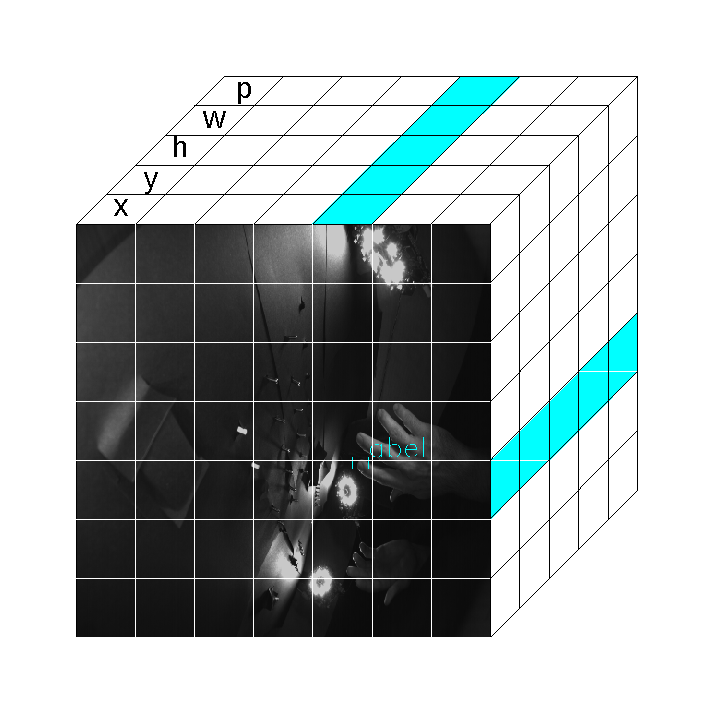
\includegraphics[width=.8\textwidth]{Kapitel/DatenPipeline/Bilder/LabelTensor.pdf}
	\caption{Label-Tensor}
	\label{img:label_tensor}
\end{figure} 
\subsection{Daten in Neuronales Netzwerk einlesen}



\newpage
%Kapitelüberschrift
\section{Architektur}
\label{chapter:architektur}
\subsection{Auswahl der Architektur}
Die Architektur wurde stark dem Yolo-Paper \cite{yolo} angelehnt. 
Dies obwohl zu diesem Zeitpunkt auch schon das Yolo v2-Paper \cite{yolo2} erschienen war.
Es gab damals schon viele gute Gründe dafür, von Beginn weg das Netzwerk und Kostenfunktionen nach dem Yolo v2-Paper aufzubauen.
So ist Yolo v2 nach dessen Paper zu urteilen schneller und genauer. 
Es wurde trotzdem Yolo v1 verwendet, weil die Beschreibung z.B. der Kostenfunktion und der Architektur im Paper von Yolo v1 um einiges genauer und verständlicher war als im Paper von Yolo v2.
Ausserdem ging man mit der Einstellung an die Arbeit, dass wenn erst das \grqq{}einfache\grqq{} Yolo v1  erfolgreich implementiert wurde, dieses entsprechend immer noch zur 2. Version erweitert werden könnte.

Das Vorgehen (Kapitel \ref{chapter:vorgehen}) aber wurde im Nachhinein betrachtet falsch angeordnet. 
So ist das Experimentieren/Optimieren eines Neuronalen Netzwerks etwas extrem Zeitaufwendiges, was man nie wirklich abschliessen kann.
So gesehen hätte das Vorgehen folgendermassen geplant werden müssen.
Sobald eine lauffähige fehlerfreie Version von Yolo v1 erreicht wurde, hätte sofort mit dem Architekturaufbau von Yolo v2 begonnen werden müssen.
Es wird davon ausgegangen, dass so noch bessere Resultate hätten erzielt werden können.

\subsection{Architekturaufbau}
\label{chapter:Architekturaubau}
\subsubsection{Hauptgraph}
\label{chapter:hauptgraph}

\begin{table}
\centering
\begin{tabularx}{1.1\textwidth}{|l|l|l|l|l|X|}
\hline
\textbf{Layer} & \textbf{Filtertyp}  & \textbf{Anzahl} & \textbf{Grösse} & \textbf{Strides} & \textbf{Output} \\
\hline 	0	& Input				&		&		&		& 448x448x1\\
\hline 	1	& Convolutional		& 64		& 7x7	& 2x2	& 224x224x64	\\
\hline 	2	& Maxpool      		& 		& 2x2	& 2x2	& 112x112x64	\\
\hline 	3   & Convolutional		& 192	& 3x3	& 1x1	& 112x112x192\\
\hline 	4	& Maxpool			& 		& 2x2	& 2x2	& 56x56x192	\\
\hline 	5	& Convolutional		& 128	& 1x1	& 1x1	& 56x56x128	\\
\hline 	6	& Convolutional		& 256	& 3x3	& 1x1	& 56x56x256	\\
\hline 	7	& Convolutional		& 256	& 1x1	& 1x1	& 56x56x256	\\
\hline 	8	& Convolutional		& 512	& 3x3	& 1x1	& 56x56x512	\\
\hline 	9	& Maxpool			&		& 2x2	& 2x2	& 28x28x512	\\
\hline 	10	& Convolutional		& 256	& 1x1	& 1x1	& 28x28x256	\\
\hline 	11	& Convolutional		& 512	& 3x3	& 1x1	& 28x28x512	\\
\hline 	12	& Convolutional		& 256	& 1x1	& 1x1	& 28x28x256	\\
\hline 	13	& Convolutional		& 512	& 3x3	& 1x1	& 28x28x512	\\
\hline 	14	& Convolutional		& 256	& 1x1	& 1x1	& 28x28x256	\\
\hline 	15	& Convolutional		& 512	& 3x3	& 1x1	& 28x28x512	\\
\hline  	16	& Convolutional		& 256	& 1x1	& 1x1	& 28x28x256	\\
\hline  	17	& Convolutional		& 512	& 3x3	& 1x1	& 28x28x512	\\
\hline 	18	& Convolutional		& 512	& 1x1	& 1x1	& 28x28x512	\\
\hline  	19	& Convolutional		& 1024	& 3x3	& 1x1	& 28x28x1024	\\
\hline  	20	& Maxpool			&		& 2x2	& 2x2	& 14x14x1024	\\
\hline  	21	& Convolutional		& 512	& 1x1	& 1x1	& 14x14x512	\\
\hline  	22	& Convolutional		& 1024	& 3x3	& 1x1	& 14x14x1024	\\
\hline  	23	& Convolutional		& 512	& 1x1	& 1x1	& 14x14x512	\\
\hline  	24	& Convolutional		& 1024	& 3x3	& 1x1	& 14x14x1024	\\
\hline  	25	& Convolutional		& 1024	& 3x3	& 1x1	& 14x14x1024	\\
\hline  	26	& Convolutional		& 1024	& 3x3	& 2x2	& 7x7x1024	\\
\hline  	27	& Convolutional		& 1024	& 3x3	& 1x1	& 7x7x1024	\\
\hline  	28	& Convolutional		& 1024	& 3x3	& 1x1	& 7x7x1024	\\
\hline 	31	& Fully-Connected	&		&(7x7x1024)x4096	&	& 4096  \\
\hline  	32	& Fully-Connected	&		& 4096x(7x7x6)	&	& 7x7x6 \\
\hline 	
\end{tabularx}
\caption{Yolo-Architektur}
\label{tbl:yolo_architektur}
\end{table}


Der grundlegende Aufbau der Architektur, wie sie letztendlich aussah kann man in der Tabelle \ref{tbl:yolo_architektur} betrachten. 
Dies sah allerdings noch nicht immer so aus.
Obwohl die Convolution-Filter schon immer in dieser Form angeordnet waren, sahen der ursprüngliche Bildinput und entsprechend die Outputs der verschiedenen Layers ursprünglich anders aus.
Nach ausführlicher Diskussion \cite{PrivateCommunication} wurde zu Beginn des Architekturdesigns entschieden, dass man nicht mit 448x448 Bildern arbeitet, wie dies im Yolo-Paper \cite{yolo} gemacht wurde.
Der Grund dafür war, dass für das Training wie auch später für den Praxiseinsatz immer 1280x960 grosse Bilder zur Verfügung standen und man entsprechend nicht Informationen \grqq{}wegwerfen\grqq{} sondern so lange wie möglich im Netz behalten wollte.
So war der Input (Layer 0 in Tabelle \ref{tbl:yolo_architektur}) damals 1280x960x1.
Entsprechend war dann auch der Output von Layer 1 nicht mehr 224x224x64 sondern 640x480x64 usw.
Da dies am Schluss nicht aufgeht mit dem Netzwerk, hatte es damals noch zwei zusätzliche Layer (29 \& 30), welche jetzt nicht mehr vorhanden sind.
Layer 29 war dabei für ein Zeropadding und Layer 30 für ein Maxpooling mit Strides 3x3 zuständig.


\begin{figure}
	\centering
	\begin{minipage}[b]{0.48\textwidth}	
		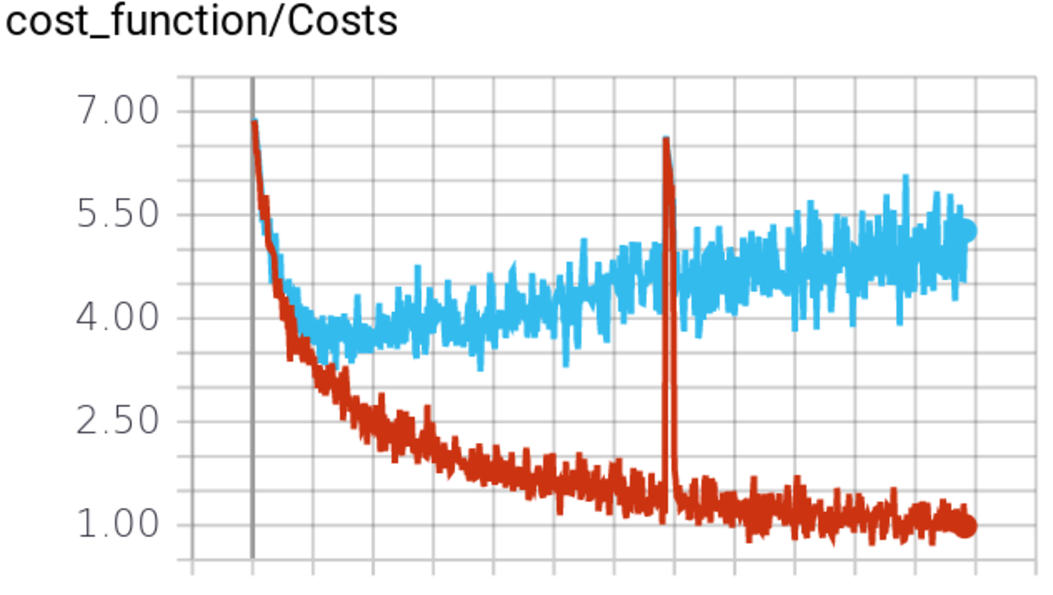
\includegraphics[width=\textwidth]{Kapitel/40Architektur/Bilder/OverflowInPretraining.pdf}
		\caption{Effekt (Extremer Anstieg der Kosten innert einer Epoche) im Pretraining. X-Achse = Zeit, Y-Achse = Kosten, Weinrot=Trainingsdate, hellblau = Validierungsdaten}
		\label{img:Overflow_pretraining}
	\end{minipage}
	\hfill
	\begin{minipage}[b]{0.48\textwidth}		
		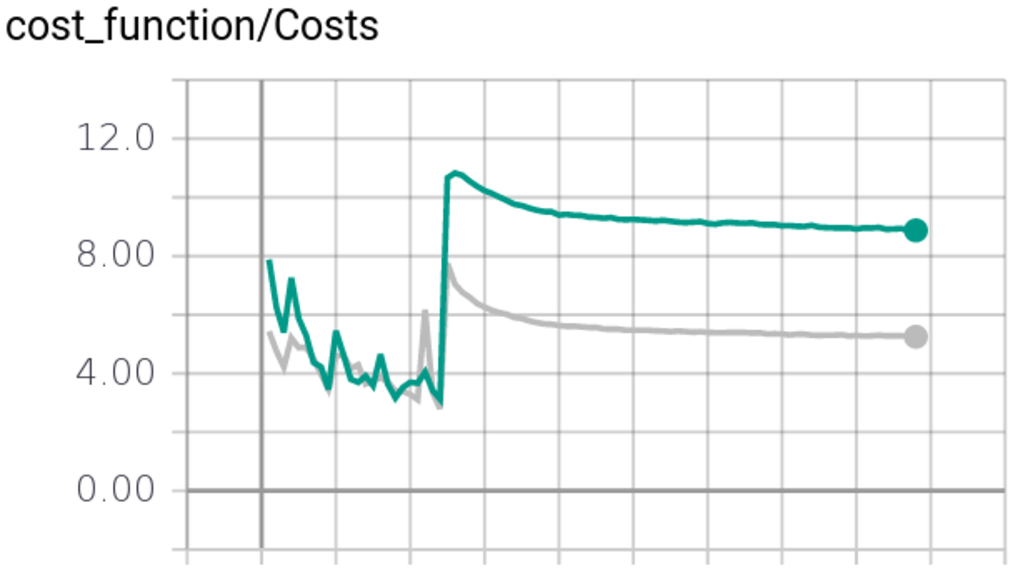
\includegraphics[width=\textwidth]{Kapitel/40Architektur/Bilder/OverflowInTraining.pdf}
		\caption{Effekt (Extremer Anstieg der Kosten innert einer Epoche) im Training. X-Achse = Zeit, Y-Achse = Kosten, grün=Trainingsdate, grau = Validierungsdaten}
		\label{img:Overflow_training}
	\end{minipage}
	
\end{figure}



Diese damalige Architektur war zu gross, um sie auch nur mit Minibatchsize=1 und Float32 ins GPU-RAM und entsprechend überhaupt zum Laufen zu kriegen. 
Entsprechend wurden alle Gewichte und Knoten mit Float16 initialisiert. 
Seit dieser Initialisierung war eine Minibatchsize=7 möglich.

Mit dieser Architektur wurde eine Zeit lang trainiert, bis sich immer mehr spezielle Effekte (siehe Abbildung \ref{img:Overflow_pretraining} \& \ref{img:Overflow_training}) im Training, wie auch im Pretraining (Details zum Pretraining im Kapitel \ref{chapter:Pretraining}) häuften.
Es konnte auch nach längerer Analyse nicht abschliessend geklärt werden, was die Ursache für diese Effekte  war.
Die Vermutung lag jedoch darin, dass es sich um Overflow-Probleme im Zusammenhang mit den verwendeten Float16 handeln könnte.
Entsprechend wurde die Architektur umgebaut, sodass die Input-Bilder künstlich verkleinert wurden, um im Gegenzug dafür Float32 verwenden zu können.
In diesem Schritt war es naheliegend, dass man sich gleich den originalen Werten, wie sie von Yolo \cite{yolo} verwendet wurden annäherte.
Entsprechend wurden die Input-Bilder auf 448x448 verkleinert.
Dies hatte wiederum zur Folge, dass seit diesem Zeitpunkt sogar eine Minibatchsize=24 verwendet werden konnte.
Ausserdem, und dies war noch viel wichtiger, traten die genannten speziellen Effekte (Abbildung \ref{img:Overflow_pretraining} \& \ref{img:Overflow_training}) weder im Pretraining noch im Training je wieder auf. 

\begin{table}
\centering
\begin{tabularx}{\textwidth}{|X|l|l|l|}
\hline  Beschreibung & Anzahl & in Bytes(Float16) & in Bytes(Float32)\\
\hline  Gewichte											& 206 M 	& 413 MB 	& 827 MB		\\
\hline  Knoten:Input=1280x960 							&  98 M 	& 186 MB 	&			\\
\hline  Knoten:Input=1280x960 Minibatchsize=7, GPU-RAM voll	& 689 M 	& 1.38 GB 	& 			\\
\hline  Knoten:Input=448x448 							&  16 M 	& 			& 64M 		\\
\hline  Knoten:Input=448x448, Minibatchsize=24, GPU-RAM voll	& 384 M 	& 			& 1.54GB 	\\
\hline
\end{tabularx}
\caption{Anzahl Gewichte und Knoten}
\label{tbl:anzahl_gewichte_knoten}
\end{table} 

Aus dieser Erfahrung kann man ableiten, dass bei Convolutional-Neural-Networks die Grösse der Input-Bilder mehr ins Gewicht fallen als die Anzahl Gewichte. 
Dies scheint nachträglich auch logisch, denn die Bilder werden während dem \grqq{}flow\grqq{} durch das Netzwerk mehrmals zwischengespeichert.
In der Tabelle \ref{tbl:anzahl_gewichte_knoten} dargestellt ist die Berechnung der Anzahl Gewichte und der Anzahl Knoten unter der Annahme, dass jedes Bild zwischen den Layern einmal als Knoten abgespeichert wird.
Dabei wurde nicht berücksichtigt, dass es pro Layer mehrere Einheiten von Knoten geben kann, wie z.B. vor und nach der Aktivierungsfunktion, Batchnorm, etc. 
Auch ohne diese zusätzlichen Layer kann man aber deutlich erkennen, dass wenn man die Minibatchsize solange erhöht, bis das GPU-RAM (im Rahmen dieser Arbeit 16GB) voll ist, viel mehr Speicher für Knoten benötigt wird als für Gewichte.

\subsubsection{Minibatchnorm}
Zu Beginn des Trainings gab es immer wieder das Problem von vanishing Gradients. Das bedeutet, dass die Gradienten im Verlauf der Backpropagation immer kleiner wurden, bis sie nur noch gleich Null waren.
Um diesem Problem entgegenzuwirken, wurde die relativ junge Allzweckwaffe der Minibatch-Normalisierung angewandt.
Dabei wird in jedem Convolutional Layer direkt nach dem Convolutional-Filter der Ausgang über den ganzen Minibatch normiert.
Es wurde auch ausprobiert die Minibatchnorm nach der Relu (Kapitel \ref{chapter:aktivierungsfunktion}) einzusetzen, anstelle von davor.
Allerdings waren die Ergebnisse der Kostenfunktion bei der Anordnung in Abbildung \ref{img:Conv-Layer} ein wenig besser.
Die Verbesserung war allerdings nur sehr klein.
Es ist nach je einem vergleichbaren Trainingslauf aber schwierig zu sagen, ob dies Zufall war, oder ob die eine Variante immer besser sein sollte als die andere.
Eine saubere statistische Aussage zu diesem Punkt war im Rahmen dieser Arbeit aber nicht das Ziel.

Seit dem Einsetzen der Minibatchnorm war das Netzwerk hervorragend in der Lage die Gradienten per Backpropagation bis zum Eingang des Netzwerks zurück zu tragen. 

\subsubsection{Aktivierungsfunktion}
\label{chapter:aktivierungsfunktion}
\begin{figure}
	\centering	
	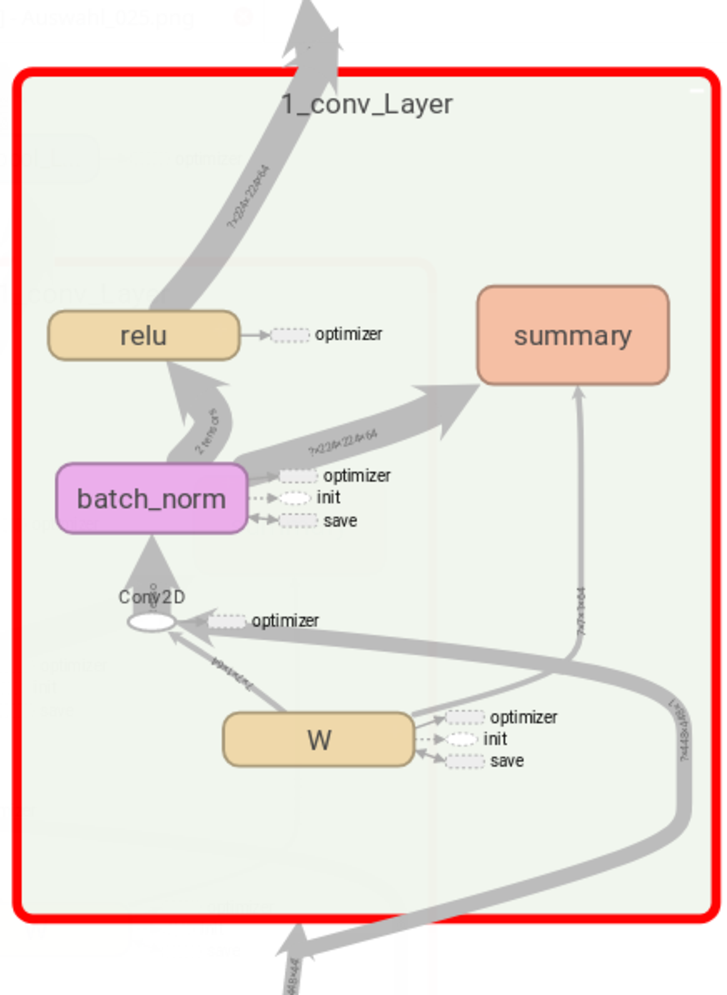
\includegraphics[width=0.5\textwidth]{Kapitel/40Architektur/Bilder/GraphProLayer.pdf}
	\caption{Aufbau eines Convolutional-Layers}
	\label{img:Conv-Layer}
\end{figure}

Wie in Abbildung \ref{img:Conv-Layer} ersichtlich, wurde als Aktivierungsfunktion eine simple Relu (Rectified Linear Unit) verwendet. Dies obwohl in yolo v1 eine leaky Relu verwendet wurde.
Der Grund für diesen Wandel war, dass seit dem verwenden der Minibatchnorm eine leaky Relu dieselbe Performance an den Tag legte wie eine normale Relu.

\subsubsection{Dropout}
Es wurde im Rahmen dieser Arbeit zur Optimierung viel mit Dropout experimentiert.
So wurde Dropout in allen, nur in den letzten, nur in den fully-connected Layer oder auch in gar keinem Layer getestet.
Die beste Performance wurde erreicht, wenn entweder nur in den letzten paar Layern oder auch nur in den fully-connected Layern Dropout eingesetzt wurde.
Wurde Dropout in allen Layern angewandt, war das Resultat massiv schlechter.

Wichtig zu wissen: Wenn man Dropout in Convolutional Layern anwendet, sollte darauf geachtet werden, dass man nicht nur einzelne Knoten von Dropout \grqq{}ausknipsen\grqq{} lässt, sondern ganze Featuremaps.
Der Grund dafür liegt darin, dass man mit der ursprünglichen Philosophie von Dropout eigentlich Gewichte zwischenzeitlich ausschalten möchte.
Bei Fullyconnected Netzwerken ist dies problemlos möglich, indem man Knoten zufällig auf Null setzt, womit automatisch die zugehörigen Gewichte ausgeschaltet wurden. 
In Convolutional Neural Networks hingegen werden die Gewichte nicht ausgeschaltet, indem man einen Knoten ausschaltet.
Dies, weil die Gewichte über die Bilder oder Feature-Maps geschoben werden und nicht einzelnen Knoten zugeteilt sind.


\subsection{Fazit}
Was die Architektur angeht, kann man aus dieser Arbeit die folgenden Punkte lernen:
\begin{enumerate}
\item Wenn in Convolutional Neural Networks Speicherknappheit ein Problem ist, sollte entweder die Tiefe des Netzwerks (weniger Layer = weniger Knoten) oder der Input verkleinert (= ebenfalls weniger Knoten) werden. 
Nicht aber sollte man zu weit von der Norm abweichen, sodass man sich was Datentypen angeht ausserhalb des Tensorflow-Standardbereichs aufhält.

\item Wenn man eine Architektur nach einer bestimmten Vorlage aufbaut, sollte erst optimiert werden, wenn man eine lauffähige fehlerfreie Version hat.
Somit kann jederzeit auf diese lauffähigen Version zurückgegriffen werden.

\item Zu Beginn des Trainings stürzte das Programm öfters ab.
Dabei war die Fehlermeldung jeweils, dass \grqq{}NAN\grqq{} (Not a Number) oder \grqq{}Infinity\grqq{} ins Tensorboard gespeichert werden sollte.
Seit die Gradienten auf $\pm 5$\footnote{\label{gradientclipping} Im Normalfall wird gemässe Deeplearning-Buch \cite{deeplearning} ein Gradientclipping von $\pm 5$ angewendet. Entsprechend wurde dies ohne weitere Recherche / Überprüfung so übernommen.}  begrenzt wurden, trat dieses Problem nie mehr auf.
Daraus folgt: Gradient Clipping ist sehr zu empfehlen, da es nicht schadet aber allfällige Probleme fernhalten kann. 
\end{enumerate}






\newpage
%Kapitelüberschrift
\section{Kostenfunktion} 
\subsection{Erster Wurf}
\label{chapter:erster_wurf}
In einem ersten Wurf war das Ziel eine Kostenfunktion zu erstellen, welche so einfach wie nur möglich sein sollte. 
So sollte man schnellstmöglich ein funktionierendes Netzwerk haben, welches einfach zu debuggen ist und später Schritt für Schritt verbessert werden konnte.
Dabei sollte der Output des Netzwerks lediglich 3 Variablen umfassen. Eine, welche die x-Koordinaten des rechten Zeigefingers vorhersagt, eine, welche die y-Koordinaten vorhersagt, und eine letzte, welche die Wahrscheinlichkeit dass sich ein rechter Zeigefinger in diesem Bild befindet vorhersagt.
Die Kosten sollten dabei wie beim originalen Yolo-Netzwerk mit den kleinsten Fehlerquadraten der Distanz von Label zu Prediction berechnet werden.
Dieser Ansatz hatte überhaupt nicht funktioniert.
Die Predictions waren irgendwo im Bild und mit menschlichem Auge keine Korrelation mit den Labels ersichtlich. 

Es wurde die Hypothese erstellt, dass dies daran läge, dass man mit dem Pretraining (Details im Kapitel \ref{chapter:Pretraining}) eigentlich Hauptsächlich einen Klassifizierer \grqq{}gezüchtet\grqq{} hatte, aber für die zwei essentiellen Predictions(x-/ y-Wert) eigentlich nur eine Regression verwendet wurde.
Beim originalen Output des Yolo-Netzwerks könnte man sich vorstellen, dass das Netzwerk für jede Gitterzelle eine intuitiv eine Klassifizierung durchführt, und entsprechend den Fehler schon stark eingrenzen kann.
Aufgrund dieser Intuitiven Erklärung wurde der Plan gefasst, die Kostenfunktion stärker an der originalen Kostenfunktion zu orientieren.

\subsection{Netzwerkoutput}
Im ersten Schritt wurde der Output des Netzwerks nahezu genau nach dem Vorbild aus dem Yolo-Papers \cite{yolo} aufgebaut. 
Die einzigen Unterschiede lagen darin, dass man pro Gitterzelle nur eine anstelle von zwei Bounding-Boxen ausgibt und dass man nur eine anstelle von 10 Klassen vorhersagt. 
Damit war der Output des Netzwerks (Abbildung \ref{img:prediction_tensor}) nahezu identisch mit dem Label-Tensor (Abbildung \ref{img:label_tensor} \& Beschreibung in Kapitel \ref{chapter:label_tensor}).
Der einzige Unterschied zwischen dem Output-Tensor und dem Label-Tensor lag darin, dass jede Gitterzelle auch eine Vorhersage zur Confidence enthält. 

%Prediction-Tensor
\begin{figure}	
	\centering
	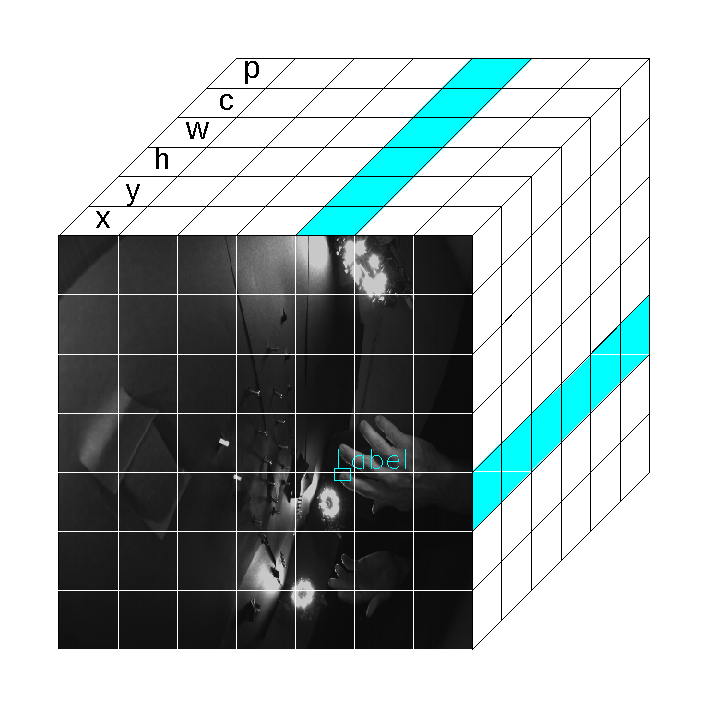
\includegraphics[width=.7\textwidth]{Kapitel/50Kostenfunktion/Bilder/PredictionTensor.pdf}
	\caption{Prediction-Tensor}
	\label{img:prediction_tensor}
\end{figure} 

Die Confidence war deshalb nicht explizit in den Labels enthalten, weil sie aus den Vorhersagen zu x, y, w und h sowie den entsprechenden Labels berechnet wurde.
Die Label-Confidence ist eigentlich nichts anderes als die IOU\footnote{\label{foot:1}IOU = Intersection Over Union} zwischen der vorhergesagten Bounding-Box und der Label-Bounding-Box einer bestimmten Gitterzelle. 
Die Berechnung der IOU aus diesen beiden Bounding-Boxen erfolgt wie aus Abbildung \ref{img:IOU} ersichtlich.

Es befinden sich allerdings in den meisten Gitterzellen keine rechten Zeigefinger. 
Aus diesem Grund existieren in diesen Gitterzellen auch keine Labels zu x,y,w und h, weshalb auch keine Label-Bounding-Boxen existieren.
In jeder dieser Gitterzellen, in welchen keine Label-Boundingboxen existieren ist die Label-Confidence automatisch=0. 
So wird man nach dem Training aufgrund der Confidence-Variable im Output für jede Gitterzelle ablesen können, ob sich darin irgend ein Objekt befindet, und wie gut dieses wahrscheinlich auf die Vorhersage von x,y,w und h passt.


%IOU
\begin{figure}	
	\centering
	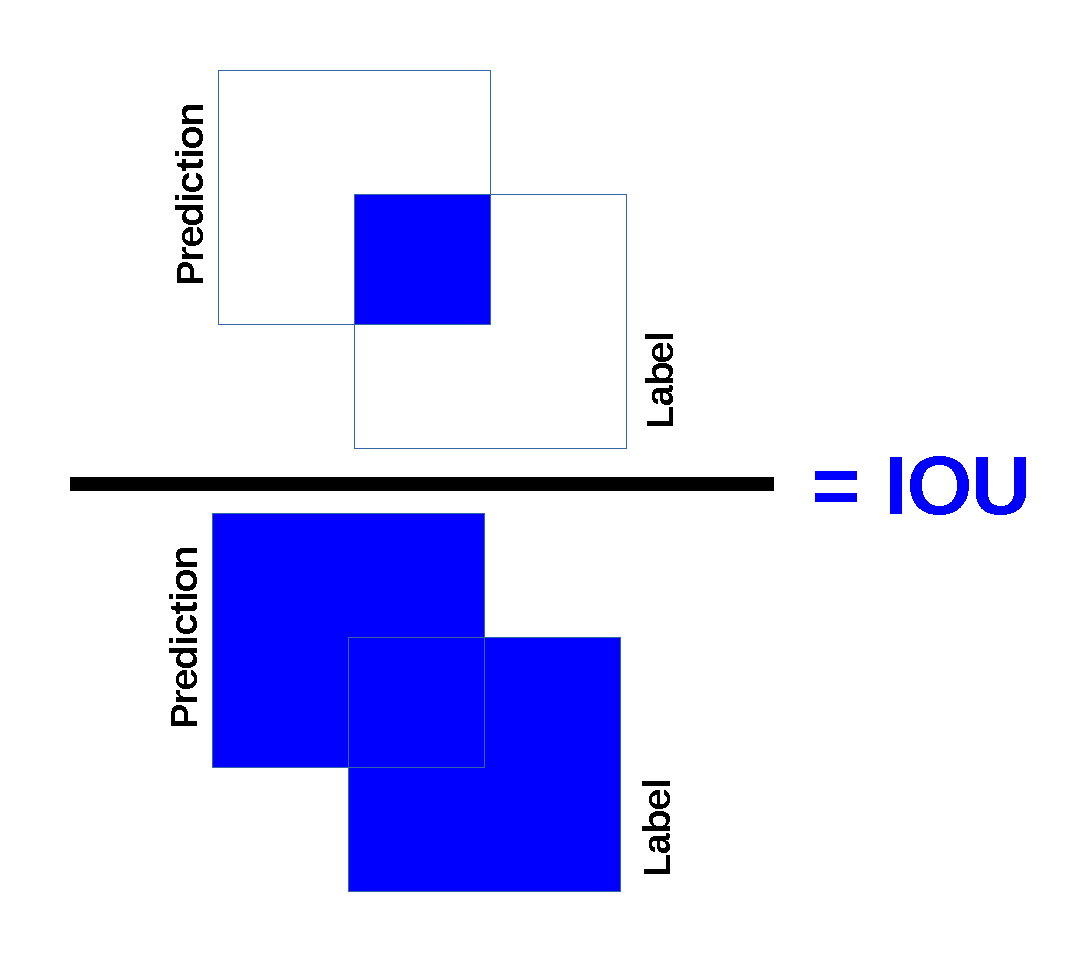
\includegraphics[width=.4\textwidth]{Kapitel/50Kostenfunktion/Bilder/IOU.pdf}
	\caption{Berechnung der IOU}
	\label{img:IOU}
\end{figure} 


\subsection{Design Kostenfunktion}
\label{chapter:design_kostenfunktion}

\begin{eqfloat}
\begin{equation}
\begin{split}
	\lambda_{coord} * \sum_{i}^{7*7}& \mathds{1}_{i}^{obj}[(x_{i}-\hat{x}_i)^{2} + (y_{i}-\hat{y}_i)^{2}] \\\
	+ \lambda_{coord} * \sum_{i}^{7*7}& \mathds{1}_{i}^{obj}[(\sqrt{w_{i}}-\sqrt{\hat{w}_{i}})^{2}+(\sqrt{h_{i}}-\sqrt{\hat{h}_{i}})^{2}] \\\
	+ \sum_{i}^{7*7}& \mathds{1}_{i}^{obj}[(C_{i} - \hat{C}_{i})^{2}] \\\
	+ \lambda_{noobj} * \sum_{i}^{7*7}& \mathds{1}_{i}^{noobj} [(C_{i} - \hat{C}_{i})^{2}] \\\
	+ \sum_{i}^{7*7}&\mathds{1}_{i}^{obj} (p_{i}-\hat{p}_{i})^{2}
\end{split} 
\end{equation}
\caption{abgespeckte Kostenfunktion wie Sie in dieser Arbeit verwendet wurde.}
\label{eq:Kostenfunktion}
\end{eqfloat}


\begin{table}
\centering
\begin{tabularx}{\textwidth}{|l|X|}
\hline  \textbf{Symbol} & \textbf{Definition}\\
\hline  $\lambda_{coord}$  & Faktor welcher verwendet wird um Fehler in den Koordinaten, sowie Höhe und Breite der Boundingboxen stärker zu gewichten. In diesem Fall wird hier ein Faktor von 5 verwendet. Diese Zahl ist so eins zu eins aus dem Yolo-Paper \cite{yolo} übernommen worden.\\
\hline  $\lambda_{noobj}$  & Faktor, welcher verwendet wird, damit der Confidence-Fehler nicht so stark gewichtet wird, wenn gar kein Objekt in dieser Gitterzelle vorhanden ist. In diesem Fall wird hier ein Faktor von 0.5 verwendet. Diese Zahl ist so eins zu eins aus dem Yolo-Paper \cite{yolo} übernommen worden.\\
\hline  $x_i$  & x-Labelkoordinaten, welche für die Gitterzelle i die Distanz vom Mittelpunkt der Boundingbox zum linken Rand der Gitterzelle i angibt.\\
\hline  $y_i$  & y-Labelkoordinaten, welche für die Gitterzelle i die Distanz vom Mittelpunkt der Boundingbox zum oberen Rand der Gitterzelle i angibt.\\
\hline  $w_i$  & Breite der Label-Boundingbox für die Gitterzelle i\\
\hline  $h_i$  & Höhe der Label-Boundingbox für die Gitterzelle i\\
\hline  $C_i$  & Label-Confidence für die Boundingbox in der Gitterzelle i\\
\hline  $p_i$  & Label-Wahrscheinlichkeit, dass sich ein rechter Zeigefinger in der Gitterzelle i befindet. \\	
\hline  $\hat{x},\hat{y},\hat{w},\hat{h},\hat{C},\hat{p}$  & Dies sind die Predictions des Netzwerks, welche den oben definierten entsprechenden Labels gegenübergestellt werden.\\
\hline  $\mathds{1}_{i}^{obj}$  & Dieses Objekt ist = 1, wenn in der Gitterzelle i ein rechter Zeigefingerspitz enthalten ist. Dieses Objekt ist = 0, wenn in der Gitterzelle i \textbf{kein} rechter Zeigefingerspitz enthalten ist.\\	
\hline  $\mathds{1}_{i}^{noobj}$  & Dieses Objekt ist = 1, wenn in der Gitterzelle i \textbf{kein} rechter Zeigefingerspitz enthalten ist. Dieses Objekt ist = 0, wenn in der Gitterzelle i ein rechter Zeigefingerspitz enthalten ist.\\
\hline $\sum_{i}^{7*7}$ & Summe über alle Gitterzellen, wobei i immer einer Gitterzelle entspricht.\\
\hline
\end{tabularx}
\caption{Beschreibung der Kostenfunktionselemente}
\label{tbl:beschr_kostenfuntion}
\end{table} 

Die Auswahl bzw. das Design der Kostenfunktion ist wahrscheinlich der wichtigste Schritt im Design eines Neuronalen Netzwerks. 
In dieser Arbeit bestand das grosse Glück, dass die Kostenfunktion grösstenteils vom Yolo v1-Paper \cite{yolo} vorgegeben wurde (Was auch mit ein Grund für die Wahl von Yolo v1 war).
Die Kostenfunktion, wie Sie in dieser Arbeit verwendet wurde kann man in Gleichung \ref{eq:Kostenfunktion} betrachten. 
Diese Kostenfunktion ist etwas einfacher als die Kostenfunktion, wie Sie im Yolo v1 Paper zu sehen ist. 
Dies hat zwei Gründe. 
Zum einen wurde pro Gitterzelle nur eine Boundingbox vorhergesagt. 
So fällt für Zeile 1-4 der Kostenfunktion das zweite Summenzeichen, sowie deren iteration über die Variable j weg. 
Zum anderen wurde nur eine Klasse(rechter Zeigefinger) gelabelt und vorhergesagt.
So fällt auf der Zeile 5 das Summenzeichen und deren entsprechende Iteration über alle Klassen weg.

Spannend war, dass es im aktuellen Fall für das Netzwerk nicht möglich war einen nach unten korrigierenden Einfluss auf die Variable $p_i$ zu nehmen.
So gingen die Vorhersagen für die $p_i$'s je länger man lernte desto stärker gegen 1.  
Der Grund dafür lag darin, dass $\mathds{1}_{i}^{obj}$ immer = 0 war, wenn \textbf{kein} rechter Zeigefingerspitz in dieser Gitterzelle enthalten ist.
So wird das Netzwerk nie korrigiert, wenn es die Wahrscheinlichkeit höher einschätzt, als sie tatsächlich ist. 
Dies stellte allerdings kein Problem dar. 
Denn die letztendliche Identifikation des Fingers, welche mit dem resultierenden Wert aus $c_i * p_i$ ermittelt wurde, war wegen der Nähe von $p_i$ zu 1 sozusagen gleichzusetzen mit $c_i$.
Da auch mit mehreren Klassen $c_i$ eine Dominante Rolle spielen würde, wenn es darum geht, ob ein Objekt erkannt wurde oder nicht, würde höchstwahrscheinlich die Performance nicht besser, wenn man Yolo mit mehr als einer Klasse trainieren würde.






 


\subsection{Fazit}
Folgende Punkte konnten aus dieser Arbeit gelernt werden, bzw. sollten im Falle einer Vertiefung beachtet werden. 
\begin{enumerate}
\item Man darf die Wahl der Kostenfunktion nicht unterschätzen. 
Wie man im Kapitel \ref{chapter:erster_wurf} sehen kann, darf man nicht annehmen, dass die Kostenfunktion frei und ohne gross nachzudenken gewählt werden kann. 
Vielmehr muss die Wahl der Kostenfunktion stark mit dem Netzwerk und dem Problem interagieren. 
\item Für die Zukunft zu beachten: In dieser Arbeit wurde pro Gitterzelle nur eine Boundingbox vorhergestagt (Dies weil die Komplexität von zwei Boundingboxen in Tensorflow nahezu jegliches Mass überstiegen hätte.). Wahrscheinlich könnte die Performance noch verbessert werden, wenn anstelle von einer min. zwei Boundingboxen pro Gitterzelle vorhergesagt würden. Dies aufgrund der Theorie \cite{PrivateCommunication}, dass mit mehreren Boundingboxen verschiedene Features eines Bildes verwendet werden können, um einen Finger vorherzusagen.
\todo[inline,size=\Large]{Dieses Fazit auf Redundanz prüfen}
\item Zum Vergleich: Im Paper Yolo v2 wurde anstelle von 7x7 Gitterzellen 13x13 Gitterzellen verwendet, was in einer höheren Präzision resultieren würde. 
Eine höhere Präzision wäre für das Endziel dieser Arbeit nur zu begrüssen. 
Wenn dies allerdings mit Yolo v1 umgesetzt würde, hätte man das Problem, dass wegen dem Grösseren Speicheraufwand, welcher für die zusätzlichen Elemente \grqq{}verbraucht\grqq{} würde die Minibatchsize verkleinert werden müsste. 
So wird angenommen, dass mit einer kompletten Umstellung auf Yolo v2 ein besseres Resultat erzielt würde, als wenn man Yolo v1 einfach erweitern würde.  
\end{enumerate}


\newpage
%Kapitelüberschrift
\section{Tests} 
\label{chapter:tests}
\subsection{Erste Ansätze}
Am Anfang ging man von der falschen Vorstellung\footnote{\label{grund_falscher_test}Der Grund für diese Fehler war, dass zu Beginn der Arbeit noch nicht von allen Variablen der Yolo-Kostenfunktion Sinn und Zweck komplett verstanden wurden. Die Erkenntnis aus diesem Fehler ist einmal mehr, dass beim Aufbau einer Arbeit auf einem bestehenden Paper dieses in noch mehr Iterationen durchgelesen werden sollte.} aus, dass die Detektion der Finger über die Variable $\hat{p}_i$ im Output des Neuronalen Netzwerks (Tabelle \ref{tbl:beschr_kostenfuntion}) läuft. 
Aus diesem Grund wurden verschiedene Tests aufgebaut.

Ein Test ermittelte aufgrund von $\hat{p}_i$ und einem beliebigen Threshold einen Status für jede Gitterzelle. Diese Status waren: 

\begin{itemize}
\item \grqq{}True-Positive\grqq{}
\item \grqq{}True-Negative\grqq{}
\item \grqq{}False-Positive\grqq{}
\item \grqq{}False-Negative\grqq{}
\end{itemize}

Dies lieferte keine brauchbaren Resultate. (siehe auch Kapitel \ref{chapter:design_kostenfunktion})
Denn wenn die Variable $\hat{p}_i$ mit andauerndem Lernen gegen 1 tendiert und nie nach unten korrigiert wird, übersteigt Sie somit irgendwann jeglichen Threshold und sagt in jeder Gitterzelle einen rechten Zeigefingerspitz voraus. 
Entsprechend ergaben die \grqq{}True-Positives\grqq{} und die \grqq{}False-Positives\grqq{} zusammen irgendwann = 1, und die \grqq{}True-Negatives\grqq{} und die \grqq{}False-Negatives\grqq{} zusammen = 0.
Somit war dieser Test gegenstandslos und man wusste, dass die Variable $\hat{p}_i$ keine Rolle spielen wird, solange nur Labels mit einem Finger verwendet wurden und entsprechend nur eine Klasse existierte.

Ein weiterer Test hatte das Ziel, dass jeweils rund um das jeweilige Label ein Kreis mit einem bestimmten Radius gelegt wurde.
Die Vorhersagen wurden aufgeteilt in Vorhersagen, welche innerhalb des Kreises lagen, und solche ausserhalb des Kreises.
Es war nur noch folgende Frage offen. 
Wie bestimmt man, welche der 7x7 Boundingboxen als \textbf{die} Vorhersage verwendet werden sollte?
Die Antwort konnte dank dem Wissen über die Aufgabe, welche das Netz erfüllen musste, relativ schnell beantwortet werden.
Denn wir wissen, dass in der Aufgabe, welche gelöst werden soll, immer nur eine rechte Zeigefingerspitze pro Bild vorhanden sein wird.
So musste dafür kein Threshold bestimmt werden, sondern es wurde diejenige Boundingbox gewählt, welche die grösste Confidence lieferte.

Mit diesem Ansatz lag ein Test vor, der tatsächlich etwas über das Resultat aussagte. 
So wurden verschieden grosse Kreise um die Labels gezogen um prozentuale Aussagen zu deren Genauigkeit zu kriegen.
Allerdings wurde relativ bald klar, dass es keinen grossen Sinn machen würde für jede Genauigkeit einen Kreis zu ziehen und diese dann einzeln auszuwerten.

Ausserdem wurde von Guido Schuster \cite{PrivateCommunication} in einem Gespräch folgende Bemerkung gemacht:
"Man sollte das Netzwerk darauf testen, worauf man es auch trainiert hatte."
Dieser Bemerkung folgte schliesslich die Schlussfolgerung, dass mit den Tests auch die IOU der Predictions gegenüber den Labels genauer betrachtet werden sollten.

\subsection{Letztendlicher Test}
\label{chapter:letztendlicher_test}
Aus den Erkenntnissen der ersten Ansätze konnte ermittelt werden, dass der optimale Output aus den Tests ein Histogram, bzw. eine Wahrscheinlichkeitsdichteverteilung sein sollte.
So konnte der Code relativ schnell so angepasst werden, dass bei einem Testlauf die Distanz von Label zu Prediction (L2-Norm) für jedes Testbild in ein Element eines Vektors gespeichert wurde.
Aus diesem Vektor konnte dann ein schönes Histogramm erstellt werden, aus welchem mit einem Blick gelesen werden konnte, wie sich die Distanzen von Predictions zu den Labels über das gesamte Testset verhielten.

Nach Fertigstellung dieses Tests war es ein Leichtes, dasselbe für die IOU anstelle der Distanz zu machen. 

Die Wahl der besten Prediction wurde ebenfalls nochmals verbessert.
Es wurde in diesem Punkt viel experimentiert und ausprobiert, obwohl in der Gleichung 1 im Yolo-Paper \cite{yolo} klar ersichtlich ist, dass für die Bestimmung der besten Prediction das Produkt aus $\hat{p}_i$ und $\hat{c}_i$ massgebend ist.
Daraus konnte gelernt werden, dass bei einem Aufbau einer Arbeit auf einem Paper dieses in regelmässigen Abständen wieder durchgelesen oder zumindest überflogen werden sollte.
Natürlich machte dies aber auch keinen Unterschied mehr.
Da $\hat{p}_i$ nahezu = 1 war, war die Prediction aus $\hat{p}_i * \hat{c}_i$ dieselbe wie wenn nur $\hat{c}_i$ verwendet wurde.

Somit war das Training des Netzwerks auf die Variable $\hat{p}_i$ sowie dessen Verwendung bisher nur irreführend und hatte keinen Nutzen.
Für die Zukunft ist es wichtig, dass dieses Yolo auch mehrere Klassen vorhersagen kann.
Dadurch macht es Sinn, diese Variable und die damit verbundenen Berechnungen in der Implementation zu belassen. 

Die Wahrscheinlichkeitsdichtefunktion, welche schliesslich bei diesen Tests durch die L2-Distanz erzeugt wurde, hatte eine etwas spezielle Form (siehe Abbildung \ref{img:dist_dichte_improved}).
Dies sorgte anfangs für Verwirrung. 
Allerdings konnte ein Gespräch mit Guido Schuster \cite{PrivateCommunication} Klarheit bringen, da es sich \grqq{}offensichtlich\grqq{} um eine Rayleigh-Verteilung handelte. 
Eine solche Verteilung entsteht, wenn zwei gaussverteilte Variablen über die L2-Norm miteinander verbunden werden.
Da genau dies im Test geschieht, war somit dieser Punkt restlos geklärt.

\subsection{Seed}
Um während den vielen Tests genaue Vergleiche zu erhalten wurde im Laufe der Arbeit ein fixer Seed implementiert und an Tensorflow übergeben.
Allerdings hatte dies zwei Tücken.
Dies waren auch die Gründe, warum dieser fixe Seed wieder aufgehoben wurde.

Die erste Tücke war, dass trotz der Übergabe eines fixen Seeds an Tensorflow, die Ergebnisse nicht reproduzierbar waren.
Offensichtlich hat es in Tensorflow noch weitere zufällige Werte, welche man auch mit einem festen Seed initialisieren müsste.
Diese wurden allerdings nicht gefunden.

Die zweite Tücke zeigte sich jedes Mal, wenn man während dem Training zwischen dem Trainingsset und dem Validierungsset hin und her wechselte.
So wurden die Bilder für das Training wieder in der genau gleichen Reihenfolge geladen wie in der letzten Epoche.
Zuerst sah es so aus, als würde der Trainingsfehler einfach in ungeheurem Tempo gegen 0 gehen, während sich der Validierungsfehler relativ schnell von jeglich Vernünftigem verabschiedete.
Allerdings wurden lediglich die ersten paar Bilder auswendig gelernt.

Der Vorteil an der zweiten Tücke war, dass man aus einem Versehen heraus sogleich überprüft hatte, ob das Netzwerk in der Lage war um overzufitten.
Es zeigte sich, dass dies der Fall war.

\subsection{Fazit}
Bei einem Neuronalen Netzwerk sollte sich früher Gedanken gemacht werden, wie man das Resultat möglichst praxistauglich testen kann.
Dies wurde in dieser Arbeit falsch gemacht.
Man hatte eine funktionierende Kostenfunktion und wollte diese nach Möglichkeit verbessern.
Allerdings ist das Ziel eines neuronalen Netzwerks nicht eine tiefe Kostenfunktion zu haben, sondern den Task, wozu es verwendet wird, möglichst gut zu erfüllen.


\newpage
\section{Resultate}

\subsection{Testvoraussetzungen}
Das Netzwerk wurde auf 1'200'000 Bildern des ImageNet-1000-class-Datasets vortrainiert.
Danach wurde es auf rund 13'900 Bildern aus dem Testaufbau \cite{TabeasFingertracking} trainiert. 
Der Test wiederum wurde auf rund 1'500 Bildern ebenfalls aus dem Testaufbau \cite{TabeasFingertracking} getestet. 
Diese Testbilder waren dem Algorithmus während des Lernprozesses nicht zugänglich und haben entsprechend keinen Einfluss auf den Lernprozess genommen. 
Ausserdem wurden diese Bilder so gewählt, dass Sie nicht gleichzeitig aufgenommen wurden. 
Dies verhindert, dass fast identische Bilder im Training und im Test vorkommen. 

\subsection{Analyse}
Um die Genauigkeit der Predictions unseres Neuronalen Netzwerkes möglichst genau beschreiben zu können wurden die zwei Werte Distanz und IOU gewählt. 
Obwohl die beiden Werte korrelieren sagt jeder für sich nicht die volle Wahrheit über die Genauigkeit der Vorhersagen aus. 
Die Distanz ist für die geplante Anwendung der wesentlichere Wert, weil diese Informationen über den Standort des Fingers im Bild preisgibt.
Die IOU ist mit der Distanz klar korreliert, denn ist die Distanz zu gross, ist die IOU schnell gleich Null. 
Sobald die Boundingbox der Prediction und die Boundingbox des Labels sich beginnen zu überlappen sagt die IOU etwas über die korrekte Vorhersage von Breite und Höhe der Boundingbox aus. Auch darüber ob die Box am richtigen Ort liegt, können aufgrund der IOU vage Annahmen getroffen werden. Aber wie gesagt, die Distanz ist dafür der sicherere Wert. 

\subsubsection{Distanz}

%Einschätzung der Distanz:
\begin{figure}	
	\centering
	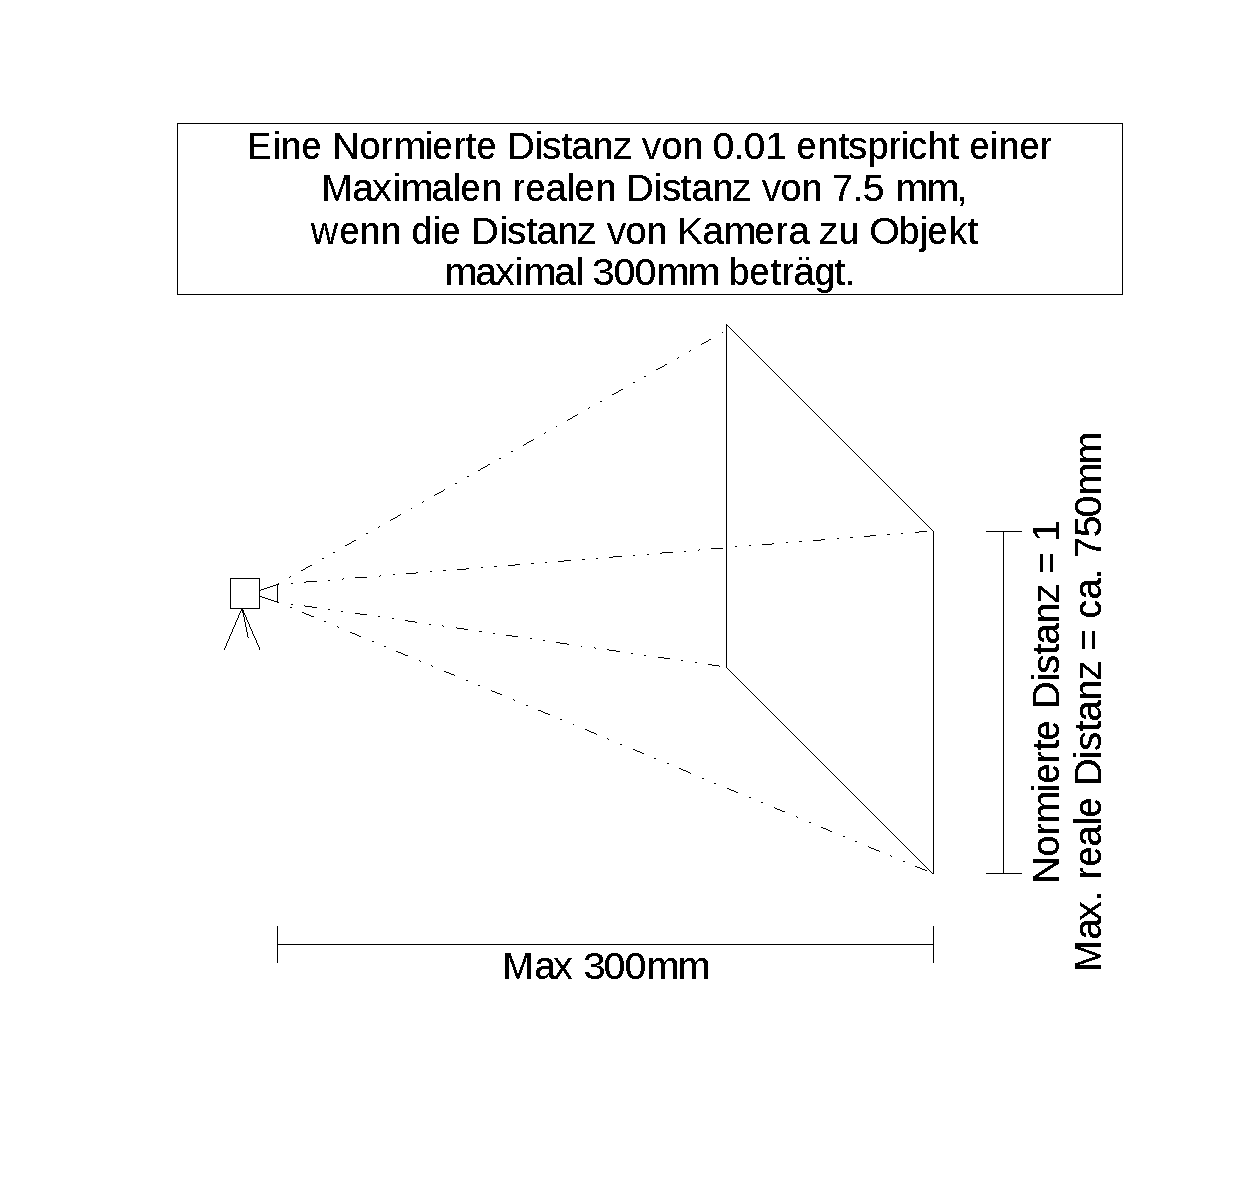
\includegraphics[width=.7\textwidth]{Kapitel/70Resultate/Bilder/DistanzenBerechnung.pdf}
	\caption{Bedeutung der normierten Distanzwerte in der realen Welt}
	\label{img:explain_normed_distance}
\end{figure}

%Beispielbilder Distanz
\begin{figure}
	\centering
	\begin{minipage}[b]{0.48\textwidth}	
		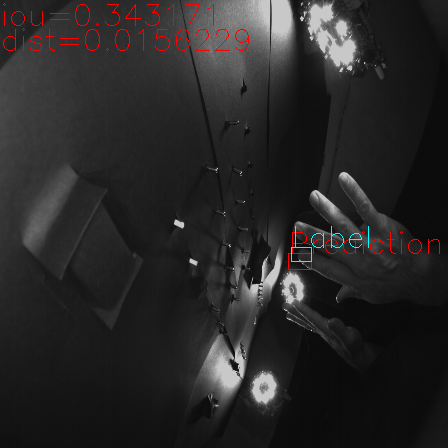
\includegraphics[width=\textwidth]{Kapitel/70Resultate/Bilder/2distKnappGut.png}
	\end{minipage}
	\hfill
	\begin{minipage}[b]{0.48\textwidth}		
		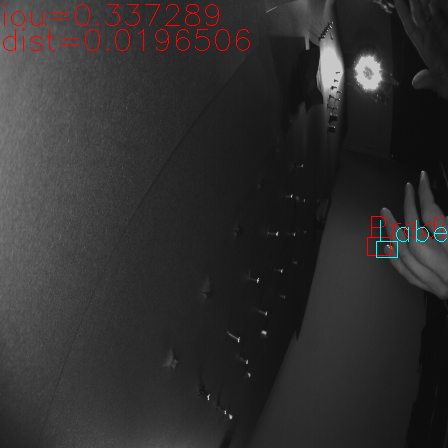
\includegraphics[width=\textwidth]{Kapitel/70Resultate/Bilder/5distKnappGut.png}
	\end{minipage}
	\caption{Prediction knapp besser als Distanz=0.02}
	\label{img:distanz_knapp_gut}
	%Eine Leerzeile einfügen	
	\begin{verbatim}
	\end{verbatim}
	\centering
	\begin{minipage}[b]{0.48\textwidth}	
		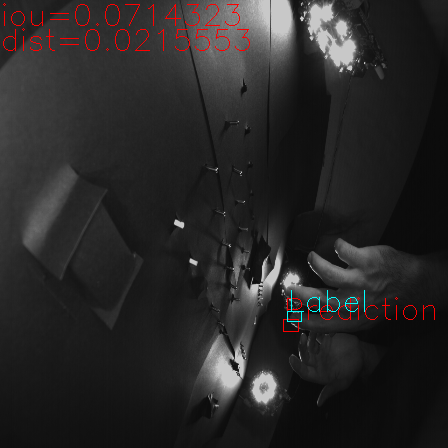
\includegraphics[width=\textwidth]{Kapitel/70Resultate/Bilder/3distKnappSchlecht.png}
	\end{minipage}
	\hfill
	\begin{minipage}[b]{0.48\textwidth}		
		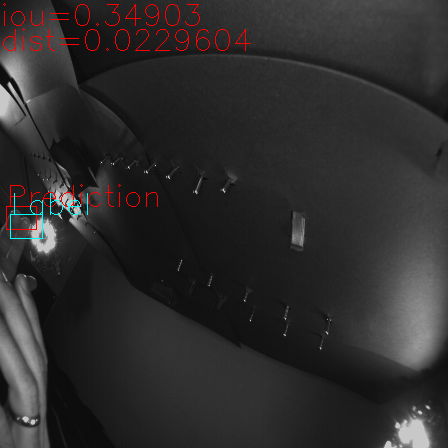
\includegraphics[width=\textwidth]{Kapitel/70Resultate/Bilder/4distKnappSchlecht.png}
	\end{minipage}
	\caption{Prediction knapp schlechter als Distanz=0.02}	
	\label{img:distanz_knapp_schlecht}
\end{figure}

%Komplette Wahrscheinlichkeits-Dichte-Funktion der Distanz
\begin{figure}	
	\centering
	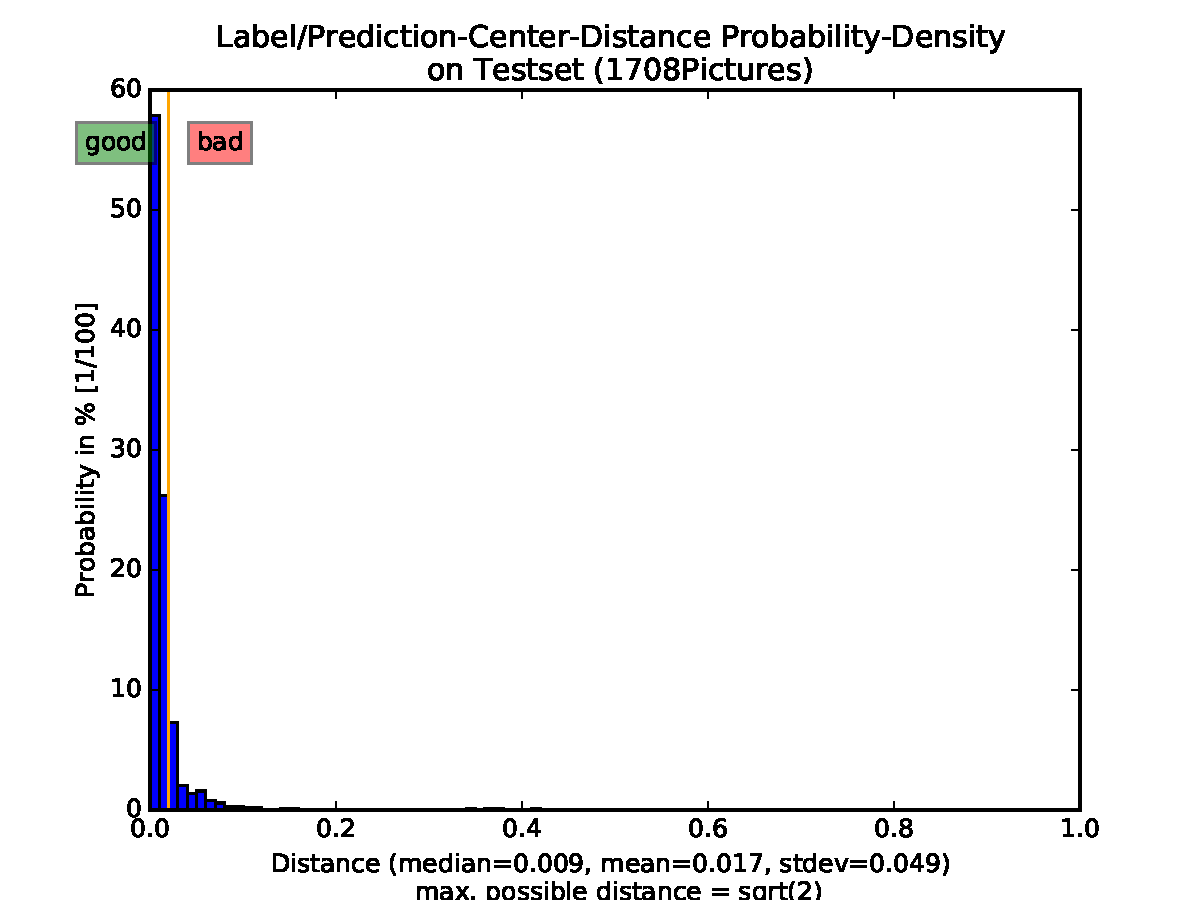
\includegraphics[width=.7\textwidth]{Kapitel/70Resultate/Bilder/distProbDensity.pdf}
	\caption{Komplette Wahrscheinlichkeits-Dichte-Funktion der Distanz (Grenze: Dist=0.02)}
	\label{img:dist_dichte}
\end{figure}
%Wahrscheinlichkeits-Dichtefunktion der Distanz. Ausreisser nicht miteingerechnet
\begin{figure}	
	\centering
	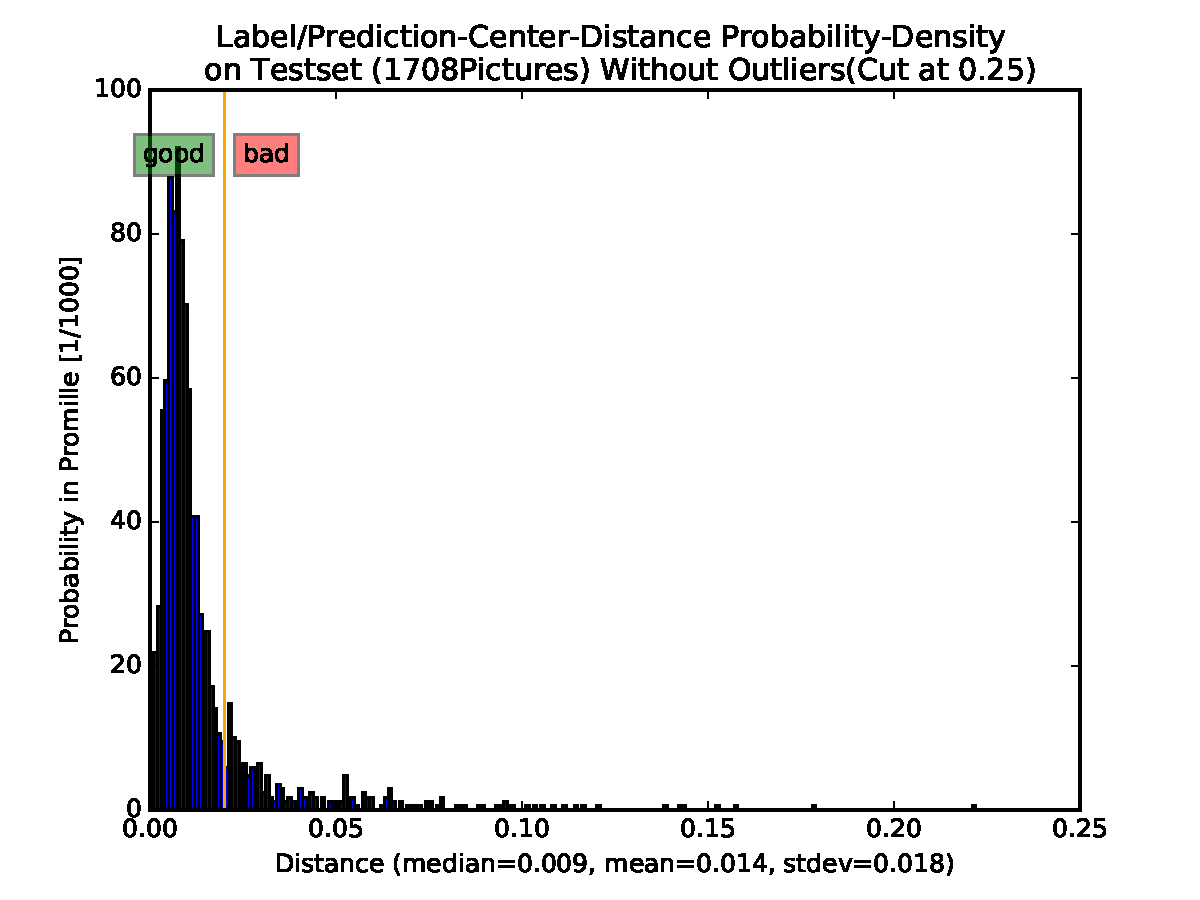
\includegraphics[width=.7\textwidth]{Kapitel/70Resultate/Bilder/distProbDensity_improved.pdf}
	\caption{Wahrscheinlichkeits-Dichtefunktion der Distanz. Ausreisser nicht miteingerechnet (Grenze: Dist=0.02)}
	\label{img:dist_dichte_improved}
\end{figure}

Die Distanz beschreibt die normierte Differenz zwischen dem Zentrumspunkt des Labels und dem Zentrumspunkt der Vorhersage. 
Sämtliche Distanzen wurden so normiert, dass die Höhe des Bildes und auch die Breite gleich eins sind. 
Die maximale Distanz zwischen zwei Punkten ist also die Diagonale über ein Bild, welche entsprechend sqrt(2) ist.
Was diese Normierten Distanzen in der realen Welt bedeuten ist auf Abbildung \ref{img:explain_normed_distance} erklärt. 
Zum Vergleich, ein Menschlicher Zeigefinger ist zwischen 10 und 20 mm breit.
Eine normierte Distanz von 0.02 entspricht auf unserem Versuchsaufbau somit ziemlich genau der Breite eines menschlichen Fingers. 

Um die Resultate in gut und schlecht einteilen zu können wurde ein Threshold von 0.02 definiert.
Die Definition dieses Thresholds wurde gemacht, indem Bilder zusammen mit der entsprechenden Distanz analysiert wurden.
Der Wert 0.02 entspricht somit derjenigen Distanz, welche gerade noch knapp annehmbar ist, um einen Finger als detektiert gelten zu lassen.
Um ein Gefühl für diese Distanzen zu kriegen lohnt es sich die Abbildungen \ref{img:distanz_knapp_gut} \& \ref{img:distanz_knapp_schlecht} anzusehen, welche Bilder zeigen, die eine Distanz nahe dieses Thresholds aufweisen. 

Um die Verteilung der Distanzen gut verstehen zu können, ist in Abbildung \ref{img:dist_dichte} eine Wahrscheinlichkeitsdichte der Distanzen im Testset zu sehen. Diese Dichtefunktion wurde erst nach der Bestimmung des Thresholds erzeugt und zeigt, dass rund 84\% der Distanzen kürzer sind als 0.02 und somit die entsprechenden Finger "erfolgreich" erkannt wurden.

Erstaunlich ist auch, dass die Distanzen, welche grösser als 0.25 sind in der Wahrscheinlichkeitsdichte in kleinen Bündeln vorkommen. 
Dies lässt darauf schliessen, dass die Trainingsdaten nicht komplett Bias-Frei sind.
Nach kurzer Kontrolle konnte tatsächlich festgestellt werden, dass z.B. bei einer Distanz von ca. 0.4 immer ein bestimmter Punkt des Hintergrundes vorhergesagt wurde, welcher tatsächlich ganz selten in den Labels als Finger markiert wurde. 

Um die Statistik nicht von Ausreissern, welche aufgrund von falschen Labels entstanden sind verfälschen zu lassen, wurde wie in Abbildung \ref{img:dist_dichte_improved} noch eine zweite Wahrscheinlichkeitsdichte-Funktion erstellt. Spannend: Der Mittelwert ist sofort um einen Drittel kleiner als zuvor. 

\subsubsection{Intersection Over Union IOU}
%Beispielbilder IOU
\begin{figure}
	\centering
	\begin{minipage}[b]{0.48\textwidth}	
		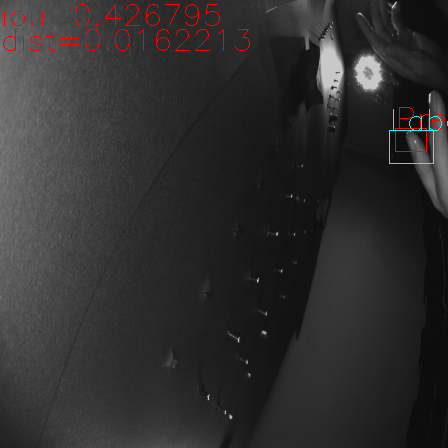
\includegraphics[width=\textwidth]{Kapitel/70Resultate/Bilder/7iouKnappGut.png}
	\end{minipage}
	\hfill
	\begin{minipage}[b]{0.48\textwidth}		
		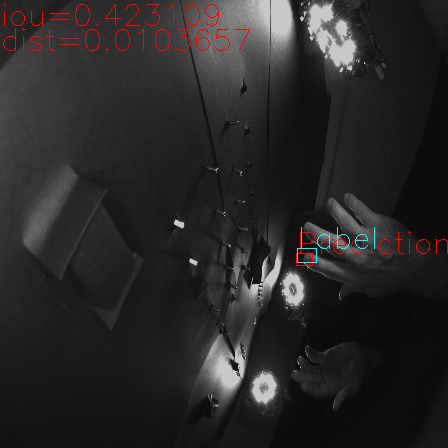
\includegraphics[width=\textwidth]{Kapitel/70Resultate/Bilder/8iouKnappGut.png}
	\end{minipage}
	\caption{Prediction knapp besser als IOU=0.4}
	\label{img:iou_knapp_gut}
	%Eine Leerzeile einfügen	
	\begin{verbatim}
	\end{verbatim}
	\centering
	\begin{minipage}[b]{0.48\textwidth}	
		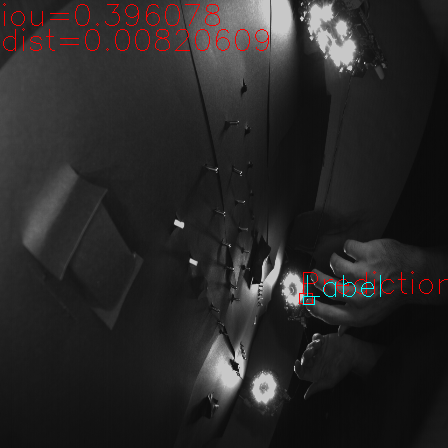
\includegraphics[width=\textwidth]{Kapitel/70Resultate/Bilder/6iouKnappSchlecht.png}
	\end{minipage}
	\hfill
	\begin{minipage}[b]{0.48\textwidth}		
		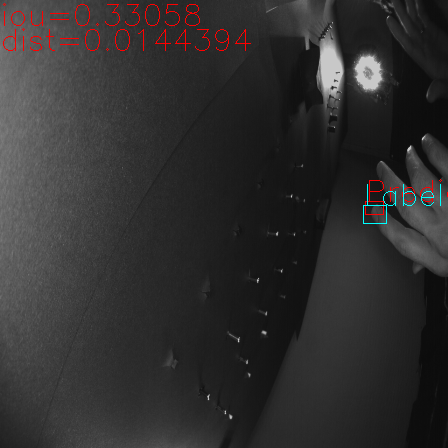
\includegraphics[width=\textwidth]{Kapitel/70Resultate/Bilder/9iouKnappSchlecht.png}
	\end{minipage}
	\caption{Prediction knapp schlechter als IOU=0.4}
	\label{img:iou_knapp_schlecht}
\end{figure}
%Wahrscheinlichkeits-Dichte-Funktion der IOU
\begin{figure}
	\centering
	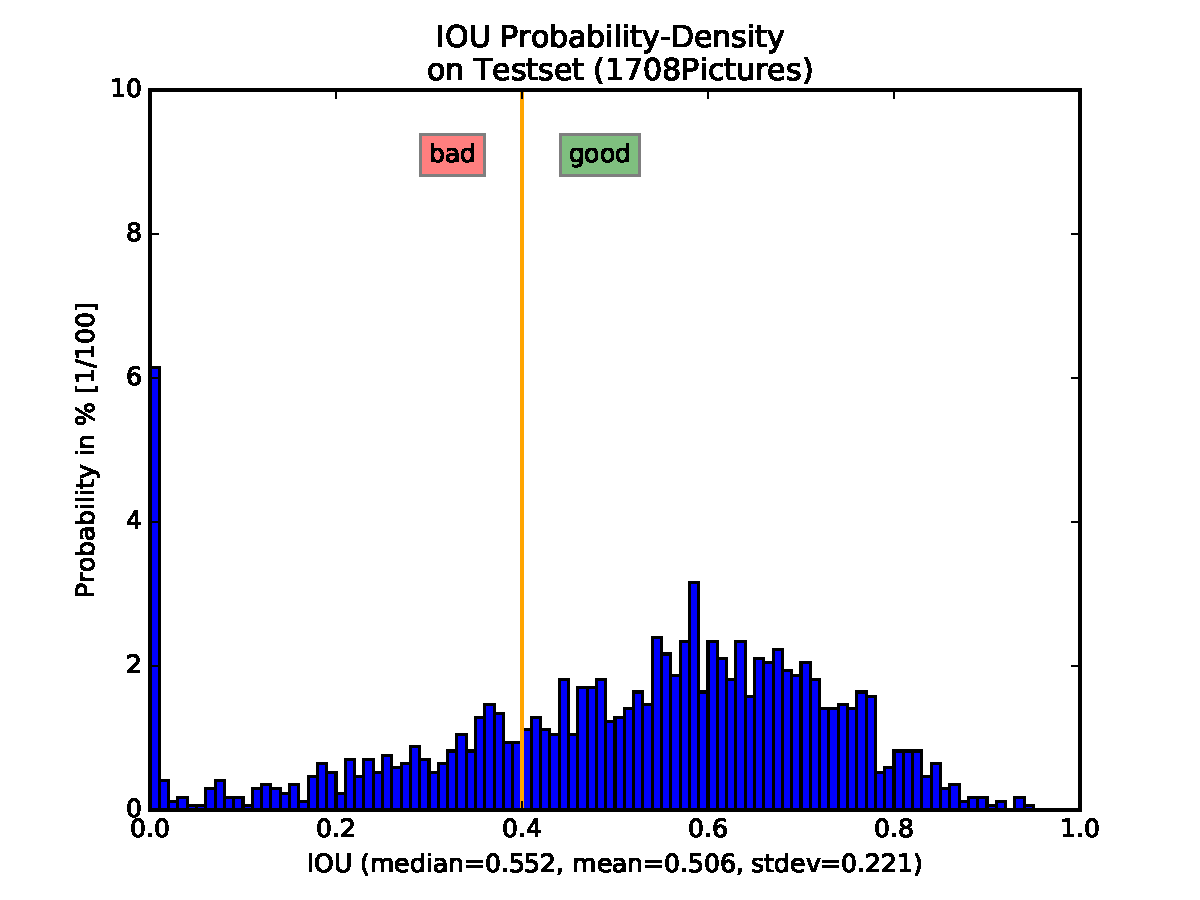
\includegraphics[width=.7\textwidth]{Kapitel/70Resultate/Bilder/IOUprobDensity.pdf}
	\caption{Wahrscheinlichkeits-Dichte-Funktion der IOU (Grenze: IOU=0.4)}
	\label{img:iou_dichte}
\end{figure}


Die IOU beschreibt die Überlappung der vorhergesagten Boundingbox und der Boundingbox des Labels. 
Daher sagt die IOU einerseits etwas über die korrekte Grösse der Boundingbox, sowie deren korrekte Lage aus. 
Um wieder etwas über gut und schlecht aussagen zu können, wurde wieder ein Threshold definiert (0.4).
Da durch die IOU wie erwähnt mehrere Faktoren beschrieben werden, ist die Grenze verschwommener. 
So gibt es nach menschlicher Ansicht hervorragende Vorhersagen, welche eine IOU von 0.3 haben und wiederum mässige Vorhersagen mit einer IOU von nahezu 0.4.
Um ein Gefühl für diesen Threshold zu kriegen lohnt es sich die Abbildungen \ref{img:iou_knapp_gut} \& \ref{img:iou_knapp_schlecht} zu berücksichtigen.
So fiel die Entscheidung den Threshold konservativ zu wählen, sodass nur Werte als gut erachtet werden könne, welche auch gut sind. 

Auch für die IOU gibt es zur Übersicht eine Wahrscheinlichkeitsdichte die in Abbildung \ref{img:iou_dichte} betrachtet werden kann.
Aus dieser Grafik kann gelesen werden, dass rund 6\% der Vorhersagen klar falsch sind, weil die IOU nur null ist, wenn sich die beiden Boundingboxen nicht berühren. Entsprechend kann gesagt werden, dass rund 94\% der vorhersagen zumindest sehr grob richtig sind, weil sich bei diesen 94\% die Boundingboxen von Label und Prediction zumindest ein ganz kleines bisschen überlappen. 


\newpage
%Kapitelüberschrift
\section{Pretraining}
\label{chapter:Pretraining}

\subsection{Daten}
Für das Pretraining des Yolo-Netzwerks wurden dieselben Daten verwendet wie im originalen Yolo-Paper \cite{yolo}.
Dabei handelte es sich um das ImageNet 1000-Klassen Wettbewerbsdatenset.
Dieses Datenset bestand aus rund 1.3 Millionen Bildern, welche alle ein Objekt aus genau 1000 möglichen Objekten enthielten.
Das Label wird über einen eineindeutigen Code im Namen identifiziert.
\subsection{Architektur}
Die Architektur, welche im Pretraining verwendet wurde (Tabelle \ref{tbl:pretraining_Architektur}) war derjenigen, welche später auch im Training (Tabelle \ref{tbl:yolo_architektur}) verwendet wurde sehr ähnlich.
So ist die Architektur der Layer von Layer 0-24 absolut identisch. 
Die Layer 25 \& 26 unterscheiden sich beim Pretraining stark vom Training, wobei die Layer 27-30 im Pretraining gar nicht vorkommen.
Was sich bei allen Layern im Pretraining vom Training unterscheidet sind die Outputs. 
Dies, weil das Input-Bild, und entsprechend auch alle Outputs im Training doppelt so gross sind wie im Pretraining. 
Der Grund dafür ist, dass dies im originalen Yolo-Paper \cite{yolo} ebenso gehandhabt und begründet wurde.

\begin{table}
\centering
\begin{tabularx}{1.1\textwidth}{|l|l|l|l|l|X|}
\hline
\textbf{Layer} & \textbf{Filtertyp}  & \textbf{Anzahl} & \textbf{Grösse} & \textbf{Strides} & \textbf{Output} \\
\hline 	0	& Input				&		&		&		& 224x224x1\\
\hline 	1	& Convolutional		& 64		& 7x7	& 2x2	& 112x112x64	\\
\hline 	2	& Maxpool      		& 		& 2x2	& 2x2	& 56x56x64	\\
\hline 	3   & Convolutional		& 192	& 3x3	& 1x1	& 56x56x192\\
\hline 	4	& Maxpool			& 		& 2x2	& 2x2	& 28x28x192	\\
\hline 	5	& Convolutional		& 128	& 1x1	& 1x1	& 28x28x128	\\
\hline 	6	& Convolutional		& 256	& 3x3	& 1x1	& 28x28x256	\\
\hline 	7	& Convolutional		& 256	& 1x1	& 1x1	& 28x28x256	\\
\hline 	8	& Convolutional		& 512	& 3x3	& 1x1	& 28x28x512	\\
\hline 	9	& Maxpool			&		& 2x2	& 2x2	& 14x14x512	\\
\hline 	10	& Convolutional		& 256	& 1x1	& 1x1	& 14x14x256	\\
\hline 	11	& Convolutional		& 512	& 3x3	& 1x1	& 14x14x512	\\
\hline 	12	& Convolutional		& 256	& 1x1	& 1x1	& 14x14x256	\\
\hline 	13	& Convolutional		& 512	& 3x3	& 1x1	& 14x14x512	\\
\hline 	14	& Convolutional		& 256	& 1x1	& 1x1	& 14x14x256	\\
\hline 	15	& Convolutional		& 512	& 3x3	& 1x1	& 14x14x512	\\
\hline  	16	& Convolutional		& 256	& 1x1	& 1x1	& 14x14x256	\\
\hline  	17	& Convolutional		& 512	& 3x3	& 1x1	& 14x14x512	\\
\hline 	18	& Convolutional		& 512	& 1x1	& 1x1	& 14x14x512	\\
\hline  	19	& Convolutional		& 1024	& 3x3	& 1x1	& 14x14x1024	\\
\hline  	20	& Maxpool			&		& 2x2	& 2x2	& 7x7x1024	\\
\hline  	21	& Convolutional		& 512	& 1x1	& 1x1	& 7x7x512	\\
\hline  	22	& Convolutional		& 1024	& 3x3	& 1x1	& 7x7x1024	\\
\hline  	23	& Convolutional		& 512	& 1x1	& 1x1	& 7x7x512	\\
\hline  	24	& Convolutional		& 1024	& 3x3	& 1x1	& 7x7x1024	\\
\hline  	25	& AveragePool		&  		& 2x2	& 2x2	& 4x4x1024	\\
\hline  	26	& Convolutional		&     	& (4x4x1024)x1000	& 	& 1000	\\
\hline 	
\end{tabularx}
\caption{Pretraining-Architektur (Ähnlich wie Training-Architektur in Tabelle \ref{tbl:yolo_architektur})}
\label{tbl:pretraining_Architektur}
\end{table}
 
\subsection{Kostenfunktion und Optimierer}
Für eine einfach Kostenfunktion wurde direkt während Pretraining aus den Bildnamen-Labels ein One-Hot-Label-Vektor mit genau 1000 Elementen erstellt.
Diesem Label-Vektor wurden nun jedem der 1000 möglichen Objekte bzw. eineindeutigen Codes ein Label-Vektor-Element zugeordnet. 
Das Label-Vektor-Element zu welchem das Bild mit seinem eineindeutigen Code als Namen gehört, wird auf 1 Gesetzt und alle anderen auf 0.
Der Output, welcher ebenfalls ein Vektor mit 1000 Elementen ist, wird nun mit dem erzeugten Label-Vektor mittels Softmax-Cross-Entropie verglichen und entsprechend die Gradienten berechnet. 

Als Optimierer wurde zuerst ein einfacher Stochastic-Gradient-Descent verwendet, welcher später durch einen Adam-Optimierer ersetzt wurde. 
Einerseits wurde im Buch Deep Learning \cite{deeplearning} empfohlen einen Optimierer mit adaptivem Momentum zu verwenden, andererseits hat sich beim ausprobieren auch einfach herausgestellt, dass die Performance von Adam gegenüber SGD massgeblich gesteigert hatte. (Abbildung \ref{img:SGDvsADAM})

Es gab allerdings auch eine Peinlichkeit im Zusammenhang mit dem Adamoptimizer.
So wurde in dieser Arbeit viel mit verschiedenen Lernraten experimentiert, wie z.B. eine regelmässige Reduktion der Lernrate nach jeweils einer bestimmten Anzahl Epochen.
Diese Experimente ergaben keinerlei verwertbare Resultate.
Der Grund dafür war, dass man den Adam-Optimizer noch nicht richtig verstanden hatte.
Denn ein zentraler Wert des Adam-Optimizers ist, dass dieser die Lernrate selber automatisch im Laufe des Trainings \grqq{}anpasst\grqq{}.
Entsprechend ist eine manuelle Anpassung der Lernrate völlig Sinnlos.

\begin{figure}
	\centering
	\begin{minipage}[b]{0.48\textwidth}	
		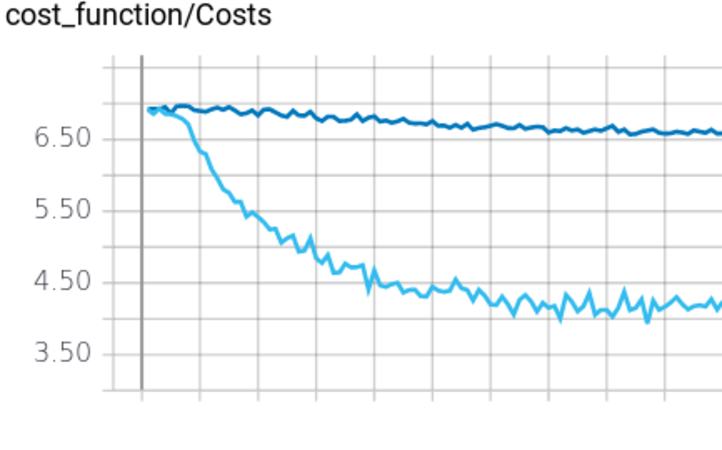
\includegraphics[width=\textwidth]{Kapitel/20Pretraining/Bilder/SGDvsADAMcost.pdf}
	\end{minipage}
	\hfill
	\begin{minipage}[b]{0.48\textwidth}		
		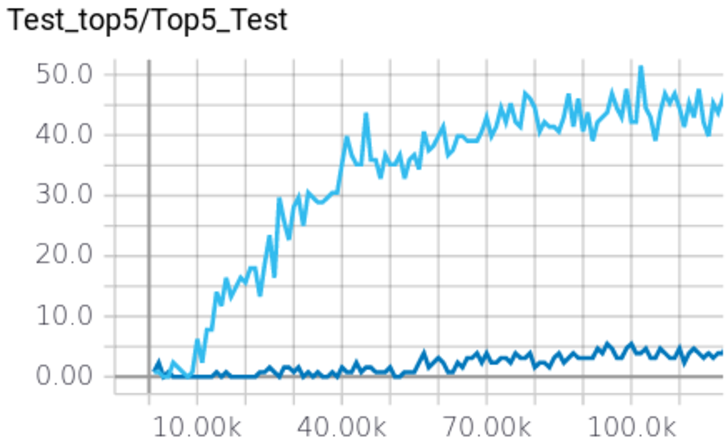
\includegraphics[width=\textwidth]{Kapitel/20Pretraining/Bilder/SGDvsADAMtop5.pdf}
	\end{minipage}
	\caption{Kosten und Top5-Test von vergleichbaren Tasks im Pretraining über einen beschränkten Zeitraum.
	links: [x-Achse=Zeit, y-Achse=Kosten]
	rechts: [x-Achse=Zeit, y-Achse=Top-5 Treffer in \%] 
	SGD=dunkelblau.
	ADAM=hellblau.}
	\label{img:SGDvsADAM}
\end{figure}
\subsection{Tests \& Resultate}
%Test Top 5 Pretraining
\begin{figure}	
	\centering
	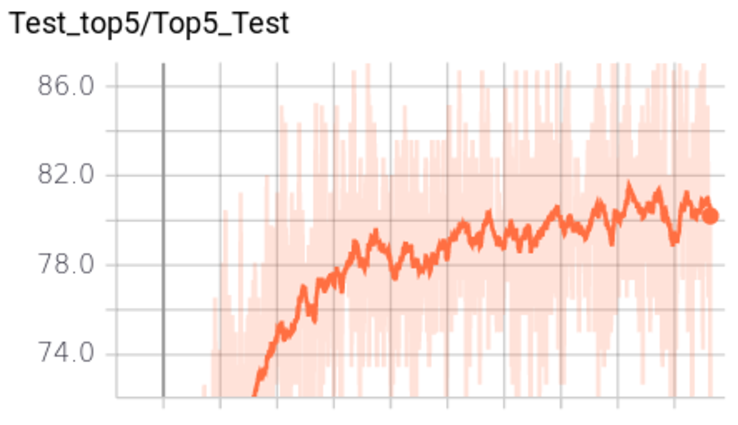
\includegraphics[width=.7\textwidth]{Kapitel/20Pretraining/Bilder/Test_top5.pdf}
	\caption{Test-Top5 nach 6 Tagen Lernzeit(x-Achse=Zeit, y-Achse=Top-5-Treffer in \%)}
	\label{img:test_top5}
\end{figure}   
Das Testen dieses Tasks war sehr einfach.
Es konnte einfach aus dem Outputvektor der Index des Elements mit dem Grössten Wert genommen und mit dem One-Hot-Index des Label-Vektors verglichen werden. 
Waren die beiden identisch, war die Vorhersage korrekt. 
Um das Resultat mit dem Resultat aus dem Yolo-Paper \cite{yolo} vergleichen zu können, wurde nicht nur der Index des höchsten Wertes im Output-Vektor verwendet, sondern gleich die Indexen der 5 höchsten Werte. 
Wie man in der Abbildung \ref{img:test_top5} erkennen kann, wurde nach 6 Tagen Lernzeit im Top5-Test im Schnitt eine Treffsicherheit von rund 80\% erreicht.
Da im originalen Yolo-Paper \cite{yolo} eine Treffsicherheit von 88\% erreicht wurde, war das Resultat dieser Arbeit um rund 8\% schlechter.

Es gibt zwei unbestätigte Vermutungen, was der Grund für diese schlechtere Performance sein könnte: 
\begin{enumerate}
\item In dieser Arbeit wurden nur Grayscaleinformationen eines Bildes verwendet, während im originalen Yolo-Paper \cite{yolo} die volle Farbinformation mitverwendet wurde. Der Grund, weshalb grayscale verwendet wurde ist, dass wir für das spätere Training ebenfalls nur Grayscale-Bilder zur Verfügung hatten.
\item Um Aufwand einzusparen wurde in dieser Arbeit nicht auf dem Image-Net Validation-Set validiert, sondern ein Teil der Trainingsdaten zum validieren verwendet. Diese Daten fehlten entsprechend im Training, was ebenfalls eine Reduktion der Treffsicherheit zur Folge gehabt haben könnte. 
\end{enumerate}
Diesen Vermutungen wurde während dieser Arbeit nicht nachgegangen.
Denn mit 80\% Genauigkeit im Top5-Test war man genügend genau, um sich erst einmal auf das eigentliche Training fokussieren zu können. 



\subsection{Gewichte}
Während dem Training wurden die Gewichte erst einmal regelmässig als Tensorflow-Gewichte-Dateien abgespeichert.
Um jedoch später möglichst flexibel zu sein wurden die besten Gewichte zusätzlich noch als Python-Objekte abgespeichert.
Dies geschah aus dem Grund, dass es zwischenzeitlich Probleme gab vortrainierte Tensorflow-Gewichte direkt ins echte Training einzulesen, wenn man nicht genau dieselbe Architektur hatte wie im Pretraining, was offensichtlich der Fall war (Siehe Tabellen \ref{tbl:pretraining_Architektur} \& \ref{tbl:yolo_architektur}).
Es gäbe zwar Tricks, wie man einen Graph aufsplitten und so die Gewichte vom Pretraining im Training verwenden könnte. 
Dieser Ansatz wurde aber nicht weiter verfolgt, weil es einerseits mit den Pythongewichten gut funktioniert hatte und andererseits, weil der Speicher der GPU's beim Training schon voll war und die Gewichte des Pretraining-Astes nicht auch noch Platz gehabt hätten.

\subsection{Fazit}
Sobald man Tensorflow grundsätzlich verstanden hat, ist das Bauen einer Klassifizierungs-Architektur eigentlich sehr einfach. 
Man muss dafür nicht einmal unbedingt die Theorie hinter dem Deeplearning verstanden haben, sondern muss einfach wissen, welche Bausteine \grqq{}man\grqq{} nimmt und wie diese angeordnet werden müssen.

Obwohl der Aufbau einer Klassifizierungsarchitektur so einfach ist, darf das Debugging nicht unterschätzt werden.
Viele Fehler sind (wenn überhaupt) erst nach mehrtägigem Training offen ersichtlich.
Entsprechend musste auch beim Test von Korrekturen jedes Mal ein bis zwei Tage gewartet werden, bis man ein Feedback bekam.
Neben Experimenten mit Lernraten, Dropout, etc., welche ebenfalls viel Zeit in Anspruch nahmen, bis ein Feedback verfügbar war, war dies der Hauptgrund für die zeitliche Verzögerungen in dieser Arbeit.

\newpage
%Kapitelüberschrift
\section{Fazit} 
\subsection{Gipshände}
Es wurde versucht eine Aussage machen zu können, ob Gipshände geeignet wären, um zukünftig Trainingsdaten zu generieren oder trainierte Netzwerke zu verifizieren.
Leider war der Hintergrund, auf den Fotos mit den Gipshänden komplett anders als in den Trainingsdaten von Yolo (schwarz abgedeckt, siehe Kapitel \ref{chapter:bilder_aufnehmen}).
Entsprechend wurde die Gipshand kaum erkannt und viel mehr völlig willkürliche Predictions gemacht.
Aus diesem Grund kann zu diesem Punkt an dieser Stelle leider keine Aussage gemacht werden.

\subsection{Yolo}
Die Genauigkeit von Yolo v1 auf Distanz und IOU ist aus menschlich subjektiver Sicht befriedigend. 
Leider aber ist die Genauigkeit noch weit vom gesteckten Ziel von 0.1 mm entfernt.
Die härtesten Gründe dafür sind:
\begin{enumerate}
\item Die Bilder müssen für Ihre Verwendung in Yolo auf eine Grösse von 448x448 geschrumpft werden. Entsprechend ist  das erreichen einer Genauigkeit unter 1mm in diesem Kontext nicht oder kaum vorstellbar.
\item Die Label-Daten hatten selber noch Fehler, die klar über 1mm lagen, entsprechend konnte es dem Netzwerk nicht möglich sein eine bessere Performance zu erlangen als dies das Trainingsset erlaubte.
\item Es wurde noch nicht alles aus dem Konzept Yolo herausgepresst, so stellt das Paper Yolo-v2 \cite{yolo2} einige Features vor, welche auch die Performance dieses Tasks verbessern könnten.
\end{enumerate}

Um auf die eigentliche Frage zurück zu kommen.
Ist Yolo, bzw. Deep-Learning im allgemeinen geeignet um die 2-D-Position von Fingerspitzen auf Bildern zu ermitteln?
Lautet die Antwort höchstwahrscheinlich Ja.
Ein Grund für diese Antwort ist, dass mit nur relativ wenigen Daten, welche sich auch als nicht allzu hochwertig herausgestellt haben mit dieser Methode trotzdem an der Grenze des möglichen gekratzt wurde.
Wieviel mehr wäre da mit hochwertigeren Daten, mehr Daten und einem verbesserten Neuronalen Netzerk möglich...


\subsection{Vorschläge für weitere Schritte}
Um in erster Instanz das Ziel eines 2-D-Fingertrackers auf Basis von Deep-Learning zu erreichen werden folgende Punkte für die Zukunft vorgeschlagen:

\begin{enumerate}
\item Bessere Daten Sammeln. 

Es gibt die Faustregel, dass man dreimal Daten aufnimmt, bis man endlich die richtigen Daten hat, um sein Netzwerk optimal zu trainieren\cite{PrivateCommunication}. 
Entsprechend sollte dabei unbedingt darauf geachtet werden, dass man mit berücksichtigt, welche Handstellen (Finger, Knöchel, Gelenke, etc.) man überhaupt braucht, damit man die Daten nicht nochmals aufnehmen muss. 
Nach dieser Projektarbeit, welche Daten aus einer Hervorragenden Masterarbeit \cite{TabeasFingertracking} verwenden durfte, ist klar, dass automatisch und maschinell erstellte Daten nicht zum optimalen Ziel führen können. 
Entsprechend sollte das Labeling von Fingern, etc. in Zukunft von Menschen gemacht werden. 
\item Mehr Daten Sammeln. 

Wie Ian Goodfellow schon in seinem Buch Deeplearning \cite{deeplearning} geschrieben hatte, wenn man alles ausprobiert hat und nichts mehr nützt, dann sammle mehr Daten. 
Entsprechend sollte bei der Generierung der Daten wie im Punkt 1 erwähnt darauf geachtet werden, dass die Daten so generiert werden, dass sie einfach per Computer vervielfältigt werden können. 
\item Die besten Stücke aus Yolo v1 und Yolo v2 herauspicken und ein optimales Netzwerk für diesen Task erschaffen. 

Für diesen Punkt sollte allerdings noch die Arbeit von Jonas Schmid \cite{HandPoseEstimation} berücksichtigt werden, weil dort höchstwahrscheinlich ebenfalls wichtige Erkenntnisse zu diesen Thema enthalten sind.
\end{enumerate}



\newpage
%sicherstellen, dass Literaturverzeichnis auch im Inhaltsverzeichnis aufgeführt wird.
\addcontentsline{toc}{section}{Literatur}
%Literaturverzeichnis anzeigen:
\bibliography{Kapitel/90Literaturverzeichnis/literatur}

\end{document}
